% Options for packages loaded elsewhere
\PassOptionsToPackage{unicode}{hyperref}
\PassOptionsToPackage{hyphens}{url}
%
\documentclass[
]{book}
\usepackage{lmodern}
\usepackage{amssymb,amsmath}
\usepackage{ifxetex,ifluatex}
\ifnum 0\ifxetex 1\fi\ifluatex 1\fi=0 % if pdftex
  \usepackage[T1]{fontenc}
  \usepackage[utf8]{inputenc}
  \usepackage{textcomp} % provide euro and other symbols
\else % if luatex or xetex
  \usepackage{unicode-math}
  \defaultfontfeatures{Scale=MatchLowercase}
  \defaultfontfeatures[\rmfamily]{Ligatures=TeX,Scale=1}
\fi
% Use upquote if available, for straight quotes in verbatim environments
\IfFileExists{upquote.sty}{\usepackage{upquote}}{}
\IfFileExists{microtype.sty}{% use microtype if available
  \usepackage[]{microtype}
  \UseMicrotypeSet[protrusion]{basicmath} % disable protrusion for tt fonts
}{}
\makeatletter
\@ifundefined{KOMAClassName}{% if non-KOMA class
  \IfFileExists{parskip.sty}{%
    \usepackage{parskip}
  }{% else
    \setlength{\parindent}{0pt}
    \setlength{\parskip}{6pt plus 2pt minus 1pt}}
}{% if KOMA class
  \KOMAoptions{parskip=half}}
\makeatother
\usepackage{xcolor}
\IfFileExists{xurl.sty}{\usepackage{xurl}}{} % add URL line breaks if available
\IfFileExists{bookmark.sty}{\usepackage{bookmark}}{\usepackage{hyperref}}
\hypersetup{
  pdftitle={Improving Land Use Change Tracking in the UK Greenhouse Gas Inventory. Report on final outputs November 2021},
  pdfauthor={Peter Levy, Sam Tomlinson, and Beth Raine},
  hidelinks,
  pdfcreator={LaTeX via pandoc}}
\urlstyle{same} % disable monospaced font for URLs
\usepackage{longtable,booktabs}
% Correct order of tables after \paragraph or \subparagraph
\usepackage{etoolbox}
\makeatletter
\patchcmd\longtable{\par}{\if@noskipsec\mbox{}\fi\par}{}{}
\makeatother
% Allow footnotes in longtable head/foot
\IfFileExists{footnotehyper.sty}{\usepackage{footnotehyper}}{\usepackage{footnote}}
\makesavenoteenv{longtable}
\usepackage{graphicx,grffile}
\makeatletter
\def\maxwidth{\ifdim\Gin@nat@width>\linewidth\linewidth\else\Gin@nat@width\fi}
\def\maxheight{\ifdim\Gin@nat@height>\textheight\textheight\else\Gin@nat@height\fi}
\makeatother
% Scale images if necessary, so that they will not overflow the page
% margins by default, and it is still possible to overwrite the defaults
% using explicit options in \includegraphics[width, height, ...]{}
\setkeys{Gin}{width=\maxwidth,height=\maxheight,keepaspectratio}
% Set default figure placement to htbp
\makeatletter
\def\fps@figure{htbp}
\makeatother
\setlength{\emergencystretch}{3em} % prevent overfull lines
\providecommand{\tightlist}{%
  \setlength{\itemsep}{0pt}\setlength{\parskip}{0pt}}
\setcounter{secnumdepth}{5}

\title{Improving Land Use Change Tracking in the UK Greenhouse Gas Inventory. Report on final outputs November 2021}
\author{Peter Levy, Sam Tomlinson, and Beth Raine}
\date{2021-11-10}

\begin{document}
\maketitle

{
\setcounter{tocdepth}{1}
\tableofcontents
}
\hypertarget{summary}{%
\chapter*{Summary}\label{summary}}
\addcontentsline{toc}{chapter}{Summary}

This report describes work on the project ``Improving Land Use Change Tracking in the UK Greenhouse Gas Inventory'' for the Department for Business, Energy \& Industrial Strategy (reference TRN 2384/05/2020). The aim of the project was to make improved estimates of land-use change in the UK, using multiple sources of data. We applied a method for estimating land-use change using a Bayesian data assimilation approach. This allows us to constrain estimates of gross land-use change with national-scale census data, whilst retaining the detailed information available from several other sources. Previous reports covered work with existing data sets (WP-A) and on developing new data sets (WP-B). This report describes subsequent work, focussed on quantifying uncertainties and improving the representation of crop-grass rotation.

The random uncertainty term \(\sigma\) for each data source has been estimated, based on agreement with the net change observed in a reference data set, comprising those data sets we believe to be most reliable for net change. The random uncertainty is now represented with both absolute and relative components, as a linear function with intercept and slope terms.

Systematic uncertainties represent biases in the data, and can be charaterised as the false positive and false negative rates (i.e.~detecting apparent change where none really occurs, and failing to detect actual change, respectively). We compared three different methods for estimating these rates, which gave similar results. These showed very high false positive rates, which mean that large corrections have to be applied to the data. The data assimilation algorithm now includes terms to account for: data-source-specific random uncertainty (sigma); data-source-specific systematic uncertainty (false positive and false negative rates); sampling error due to low survey frequency (e.g.~decadal cf.~annual); and uncertainty in extrapolation outwith (pre/post) survey time period.

Additional data sets, which were not previously available have also been included in the analysis. All the holdings-level agricultural census data available in the UK from 1990 to 2019 have now been included. The CROME data set, covering crops in England, has been added.

We have improved the accuracy of how we represent crop-grass rotations, using the idea of ``life tables'' or age-specific transition probabilities, from population modelling. The life table probabilities are based on an analysis of the data available data from IACS, CROME, LCM, and LCC, and these all show consistent patterns. Of these, IACS has much the longest time span of data, and is the dominant source of information. Using this method, the observed frequencies of transitions from crop to grassland as a function of cropland age (and v.v. for grassland) are now reproduced in the land-use vectors, and thereby approximate the observed frequency of crop-grass rotations.

Since land-use change is now represented spatially, we can separately identify that occurring on mineral soils and organic soils. In summary form, land-use vectors and the matrices of land-use change are now provided separately for mineral and organic soils for each DA.

The land-use change output data are provided as space-time data cubes at 100-m and 1000-m resolution for the period 1950-2020. These are also provided in summary (non-spatial) form as the set of unique land-use vectors, and the matrices of land-use change. In principle, many thousand samples of the posterior distribution are available (currently 20000 samples of the matrices are stored per DA). Many samples of the mapped and vector data can be provided from these, given practical computing and storage constraints, but the optimal way to produce these depends on how they are used in the LULUCF inventory work, and this is open to discussion. Storing land use as a 71-digit character string at 91 million locations (for the time period 1950-2020 at 100-m resolution) requires \textasciitilde50 MB, or \textasciitilde5MB in vector summary form, and much less at 1-km resolution.

The workflow for the project uses a ``Make''-like paradigm to maintain a reproducible workflow, implemented in the R ``targets'' package (\url{https://books.ropensci.org/targets/}). This means that the dependencies among functions and input data are analysed dynamically and stored in a hash table. Any changes to source code functions or input data are detected automatically, and only the invalidated components re-run as necessary. This has several advantages: forcing the workflow to be declared at a higher level of abstraction; only running the necessary computation, so saving run-time for tasks that are already up to date; and most importantly, providing tangible evidence that the results match the underlying code and data, and confirm the computation is reproducible. All the code is under version control on GitHub.

MCMC algorithms typically have to run for many iterations to produce an acceptable sample of the posterior, so that parameter estimates (the Beta matrices) are robust. For each year and each DA, the algorithm was run with nine MCMC chains for 200,000 iterations. Convergence was assessed by a standard method - comparing within-chain variance with among-chain variance via the Gelman-Rubin statistic. As chains move towards convergence, the value of this tends towards 1, and the standard test requires that this value is less than 1.1. This criterion is well met with this number of iterations. It is standard to discard ``burn-in'' samples prior to convergence, and to thin chains by a factor of ten to remove any autocorrelation. This yields around 16000 posterior Beta samples, which gives potentially the same number of posterior samples of the land-use vectors. However, it may be more practical to combine the calculation of fluxes into this code, without storing all the underlying data.

We produced a time series of maps describing our best estimate of land-use change given the available data, as well as the full posterior distribution of this space-time data cube. This quantifies the joint probability distribution of the parameters, and properly propagates the uncertainty from input data to final output. The output data has been summarised in the form of land-use vectors. The results show that we can provide improved estimates of past land-use change using this method. The main advantage of the approach is that it provides a coherent, generalised framework for combining multiple disparate sources of data, and adding additional sources of data is straightforward.

\hypertarget{introduction}{%
\chapter{Introduction}\label{introduction}}

This report describes work carried out on the project
``Improving Land Use Change Tracking in the UK Greenhouse Gas Inventory'' for the Department for Business, Energy \& Industrial Strategy (reference TRN 2384/05/2020). The aim of the project was to make improved estimates of land-use change in the UK, using multiple sources of data, using a Bayesian data assimilation approach. Two previous reports describe the background to the project and results from Work Package (WP) A (\href{https://nerc-ceh.github.io/luc_track/}{Levy et al.~2020}), using pre-existing data sets, and work developing new data sets based on Earth Observation in WP-B (Rowland et al.~2021).
This report describes subsequent work which focussed on assessing the uncertainties in data sets, and incorporating these in the data assimilation procedure.
Specifically, we aimed to:

\begin{itemize}
\tightlist
\item
  quantify random uncertainty in the different data sources;
\item
  quantify systematic uncertainty, i.e.~biases which may make a data source under- or over-estimate land-use change;
\item
  represent the uncertainty associated with the different sampling frequencies of the data sources (e.g.~annual versus decadal surveys);
\item
  handling the uncertainty associated with the different temporal coverage of the data sources (avoiding step changes when data coverage starts or stops);
\item
  incorporate some additional data sets which were not previously available because of data access or processing time constraints;
\item
  improve the representation of the rotational change between crop and grassland.
\end{itemize}

The above were incorporated in the data assimilation procedure, and results produced for each of the Devolved Administrations (DAs) of the UK. Land-use change on mineral soil and organic soil was estimated separately in each DA.

The remainder of this report describes these tasks and the resulting estimates of land-use change produced after their inclusion.

The first section on {[}quantifying uncertainty{]}{[}Quantifying Uncertainty in Land-Use Data Sources{]} describes how uncertainty is represented, and estimates random and systematic uncertainty by comparison with a reference data set.

The \protect\hyperlink{assessing-systematic-errors-in-estimates-of-land-use-change-sensitivity-to-survey-interval-length}{next section} describes an alternative method for systematic uncertainty based on the length of the interval between surveys.
As a third method, we then look at how errors in \protect\hyperlink{estimating-false-positive-rates-in-detection-of-land-use-change-based-on-classification-accuracy}{map classification} propagate into errors in estimates of land-use change.

Next, we describe a method for more accurately representing the frequency of rotational land-use change, using the idea of \protect\hyperlink{using-life-tables-in-modelling-land-use-change}{``life tables''} borrowed from polulation modelling.

The previous reports give detailed descriptions of the methods. However, here we reproduce the basic rationale and approach of the project for background.

\hypertarget{tracking-land-use-change}{%
\section{Tracking land-use change}\label{tracking-land-use-change}}

The tracking of land use and land-use change is fundamental to producing accurate and consistent greenhouse gas inventories (GHGI) for the Land Use, Land-Use Change and Forestry (LULUCF) sector. This is necessary to meet the international requirements of the Kyoto Protocol to the UN Framework Convention on Climate Change (UNFCCC) and the Paris Agreement and the national requirements of the UK's Climate Change Act and related legislation within the UK's Devolved Administrations.

The estimation of land-use change in the current UK GHGI is based on a combination of infrequent CEH Countryside Surveys and afforestation/deforestation statistics from the GB Forestry Commission. It uses Approach 2 (non-spatial land-use change matrices) as described in the KP Guidance. However, this matrix-based approach, and its implementation in the UK, have some important limitations. Firstly, the non-spatial matrix-based approach is insufficient for tracking annual land-use change: the matrices have no time dimension, and are defined independently each year. There is therefore no possibility of representing a sequence of land-use on the same parcel of land (such as afforestation followed by deforestation, or crop-pasture rotations). Secondly, the data used to estimate these matrices in the UK are rather limited. The CEH Countryside Surveys were only carried out approximately once per decade, and whilst the geographical extent was very wide, the actual ground area surveyed was small as a fraction of the total UK area. The afforestation/deforestation statistics from the Forestry Commission have good national coverage (excluding Northern Ireland) but do not contain any information on the spatial location or land use prior to afforestation or following deforestation.

In October 2019, the UNFCCC Expert Review of the UK 1990-2017 GHG inventory raised concerns in relation to the reporting requirements of the second commitment period of the Kyoto protocol. They questioned whether the current approach is appropriate for the identification and tracking of lands where the elected Article 3.4 activities occur (i.e.~Cropland Management, Grazing Land Management and Wetland Drainage and Rewetting). They recommended that the UK explore how to make the best possible use of available data and prepare and implement a work-plan to enable the use of these data. The UK has already explored several approaches to land use tracking, including a data assimilation approach to integrate available land-use data into land-use vectors, which was successfully piloted in Scotland (Levy et al. \protect\hyperlink{ref-Levy2018}{2018}). This project builds on that approach to assess gross land-use change, and land-use history for the whole of the UK from 1990 to 2019.

As well as improving accuracy of the GHGI, a time series of spatially explicit land-use change would enable better tracking of mitigation activities and improve baseline data for scenario modelling. These baseline data are needed for understanding the potential of land-based mitigation and adaptation options. The government's ambitions for Net Zero by 2050 or sooner means that the LULUCF sector will have an increasingly critical role in the UK's overall GHG balance. This kind of scenario modelling will become very important to inform the setting of future carbon budgets and monitor progress towards the UK's legal obligations to GHG emissions reductions. An accurate spatio-temporal land-use change data set would be useful to other stakeholders and UK government departments. For example, from the perspectives of biodiversity conservation, air quality, or ecosystem services, there are clear applications of these data for understanding and tracking the effects of land use.

\hypertarget{approach}{%
\section{Approach}\label{approach}}

If we had reliable maps of land use each year, we could infer land-use change by difference. However, even with advances in satellite sensors, GIS and spatial data handling, the accuracy of change detection from EO-based products is generally too poor to do this; the different EO products are inconsistent (with each other, and with themselves over time), irregular, and become more infrequent as we go back in time.
Change is more reliably detected by repeat gound-based surveys, but these have other short-comings. For example, the annual June Agricultural Census gives a long record of areas in different land uses, but does not provide spatial data, or any information on gross change (i.e.~what land uses have changed to which other land uses). The CEH Countryside Survey did provide spatial data with gross change, but without complete coverage, and only at infrequent intervals.

In light of the above, some data assimilation method, which combines the spatio-temporal data with non-spatial repeat survey data, would appear to provide a solution. To this end, we previously developed a methodology using a Bayesian data assimilation approach, and this has been applied successfully to Scotland (Levy et al. \protect\hyperlink{ref-Levy2018}{2018}). This method allowed for the use of a wider range of data types, including high-resolution spatial data, and combined them in a mathematically coherent way. Importantly, the method produced the appropriate data structure needed for modelling the effects of land-use change on GHG emissions - the set of unique land-use vectors (i.e.~unique sequences of land use, or land-use histories) and their associated areas. An important feature is that the uncertainty in land-use change can be easily propagated to provide the uncertainty in GHG emissions, because the procedure explicitly handles the distribution of plausible vectors of land-use change.
The approach provides a general framework for combining multiple disparate data sources with a simple model which describes how these data sources inter-relate. This allows us to constrain estimates of gross land-use change with reliable national-scale census data, whilst retaining the detailed spatial information available from several other sources. Here, we apply this methodology to improve and update the tracking of land-use change for the UK. Our aim was to apply a Bayesian approach to make spatially- and temporally-explicit estimates of land-use change in the UK, using multiple sources of data.

All the code is written in R using the ``literate programming'' paradigm implemented with Rmarkdown, which combines the source code, text/graphical output, documentation, and report text within the same document. This ensures integrity of documentation, code and corresponding outputs. All the Rmarkdown files are held in a GitHub repository, for version control and wider accessibility. The documentation is rendered using bookdown and made publicly available as a \href{https://nerc-ceh.github.io/luc_track/}{web site via GitHub Pages}. This documentation describes the data processing workflow so as to make it reproducible.

\hypertarget{quantifying-random-uncertainty-in-land-use-data-sources}{%
\chapter{Quantifying Random Uncertainty in Land-Use Data Sources}\label{quantifying-random-uncertainty-in-land-use-data-sources}}

\hypertarget{introduction-1}{%
\section{Introduction}\label{introduction-1}}

Several different data sources provide observations of the transition matrix \(B\) and the net and gross changes in area of each land use (\(D, G, L\)). The method used in WP-A treated all these data sources as equally uncertain, and assumed the same relative error for all observations. However, in reality, we know that these data sets have different levels of uncertainty: some data sets are closer to direct observations, are more plausible, and we have greater faith in these. We want to reflect this in the methodology by quantitatively associating different uncertainties with each data set. This is straightforward in principle, but there are several considerations when doing this in practice:

\begin{enumerate}
\def\labelenumi{\arabic{enumi}.}
\item
  We can consider increasing levels of detail:

  \begin{itemize}
  \item
    variable-specific uncertainties (i.e.~different for \(B, G, L\) \& \(D\))
  \item
    data source type-specific uncertainties (i.e.~different for ground-based vs EO data)
  \item
    data set-specific uncertainties (i.e.~different for CS, IACS, LCM etc.)
  \item
    land-use type-specific uncertainties (i.e.~different for woods, crops, grass etc.)
  \item
    time-specific uncertainties (i.e.~different for 1990, 2000 \ldots{} 2019)
  \end{itemize}
\item
  Rather than continuous data with a simple \(\sigma\) error term, the \(B\) observations are count data in a 6 x 6-way classification. When considering land-use \emph{change}, we can compare the 36 elements of this classification from one data source with another (or the truth), so we have a 36 x 36 error matrix (or ``confusion'' matrix). Various metrics can be calculated which summarise the agreement measured by this matrix.
\item
  We can specify uncertainty with greater or lesser rigour: there are several possibilities for how we represent ``uncertainty'' in the mathematical model.
\item
  We can estimate uncertainty subjectively, or base it more closely on data. There are also several possibilities for how we translate measures of uncertainty in the data in to the mathematical model.
\end{enumerate}

A limitation is that none of the data sources represents absolute truth, and we have no definitive data set against which to calibrate.

\hypertarget{representation-of-random-uncertainty}{%
\subsection{Representation of random uncertainty}\label{representation-of-random-uncertainty}}

The data sources are assimilated in the Bayesian method via the likelihood function, which includes a term \(\sigma^{obs}\), representing the standard deviation in the probability density function for the observation. The observation is thus not assumed to be the true value, but subject to errors which make it deviate from this. Random uncertainty is represented by the magnitude of \(\sigma^{obs}\) - large values of \(\sigma^{obs}\) represent high uncertainty (systematic uncertainty is considered in later Sections).
For each observation, a likelihood is calculated, assuming that measurement errors show a Gaussian distribution and are independent of each other.
In mathematical notation, the likelihood of observing the area changing from land use \(i\) to land use \(j\), \(\beta_{ij}^{\mathrm{obs}}\), is

\begin{equation} \label{eq:likBeta}
 \mathcal{L} = \frac{1}{\sigma_{ij}^\mathrm{obs} \sqrt{2\pi}} \mathrm{exp}(-(\beta_{ij}^{\mathrm{obs}} - \beta_{ij}^{\mathrm{pred}})^2/2 {\sigma_{ij}^\mathrm{obs}}^2)
\end{equation}

where \(\beta_{ij}^{\mathrm{pred}}\) is the corresponding prediction, and \(\sigma_{ij}^\mathrm{obs}\) is the uncertainty in the observation. There are analagous terms for \(G, L\) and \(D\) which can all be multiplied. For example, the term for the likelihood of observing the net change in land use \(u\), \(D_{u}^{\mathrm{obs}}\), is

\begin{equation} \label{eq:likNet}
 \mathcal{L} = \frac{1}{\sigma_{u}^\mathrm{obs} \sqrt{2\pi}} \mathrm{exp}(-(D_{u}^{\mathrm{obs}} - D_{u}^{\mathrm{pred}})^2/2 {\sigma_{u}^\mathrm{obs}}^2)
\end{equation}

We previously assumed that \emph{relative} measurement uncertainty was the same for all observations, i.e.~a constant proportion of the observed value. Thus, observations of large areas come with larger absolute uncertainty. Here, we estimate more specific uncertainties \(\sigma^\mathrm{obs}\) for the different data sources, and potentially this can be extended to be specific for each individual observation.

Two additional issues concern the specification of the random uncertainty when accounting for the effects of the frequency of surveys, and avoiding step changes when data sets begin and end. For example, Countryside Survey data come from approximately decadal surveys, but are interpolated and used as if they were constant annual values within each decade. We incorporated some simple methods to include these effects appropriately.

\hypertarget{methods}{%
\section{Methods}\label{methods}}

\hypertarget{estimating-sigmamathrmobs-from-reference-data}{%
\subsection{\texorpdfstring{Estimating \(\sigma^\mathrm{obs}\) from reference data}{Estimating \textbackslash sigma\^{}\textbackslash mathrm\{obs\} from reference data}}\label{estimating-sigmamathrmobs-from-reference-data}}

A pre-cursor step is to define a reference data set with which we compare each data source. In the absence of ideal ground-truth data, some subjectivity is inevitable here, and we use the data sets which we believe to be the most plausible or closest to the truth, based on judgement and prior knowledge. For agricultural land, we defined the reference data set as the June Agricultural Census data for crops, grass and rough grazing, as this is has a very long record and is submitted annually as part of reporting to FAO.
For forests, the pre-existing record of afforestation and deforestation based on FC statistics was used, as this is also long-running and has been submitted as official national data.

We applied a simple method, basing all the \(\sigma^\mathrm{obs}\) terms on the ``lowest common denominator'' data set, the time series of net area change \(D\). Although they vary in the higher levels of detail, all data sources produce estimates of \(D\), so we can calculate a comparable metric of agreement across all data sets. Suitable metrics are the root-mean-square error (RMSE), mean-absolute error (MAE) and the correlation coefficient.
We used the RMSE and the correlation coefficient, as measures of absolute and relative agreement, respectively.
We multiplied these (rescaling the correlation coefficient as \(1/(r^2+1)\)) to give a single scaling factor for \(\sigma^\mathrm{obs}\) (``CV'' in the table).
This metric is used as a scaling factor in estimating \(\sigma^\mathrm{obs}\), such that data sources with poor agreement receive high \(\sigma^\mathrm{obs}\) (high uncertainty). Some subjectivity comes into which metrics to use, and the absolute values of \(\sigma^\mathrm{obs}\), but the relative uncertainties (and therefore weighting) are based quantitatively on data.

\hypertarget{effects-of-survey-frequency-and-survey-startstop-dates}{%
\subsection{Effects of survey frequency and survey start/stop dates}\label{effects-of-survey-frequency-and-survey-startstop-dates}}

Each pair of surveys gives an estimate of land-use change over some time interval.
When survey observations are not available annually, we are effectively trying to estimate the change in a population (all years) from a sample (the years when surveys were carried out).
Using the analogy with conventional sampling theory, the standard error in our estimate should be lower in more frequent surveys, because more samples are included.
We can apply the same logic to infer the appropriate correction to apply to \(\sigma^\mathrm{obs}\), such that it reflects the uncertainty about the rate of land-use change in any given year within the inter-survey interval:

\begin{equation} \label{eq:sigma_ann}
  \sigma_\mathrm{ann}^\mathrm{obs} = \sigma^\mathrm{obs} \sqrt{n}
\end{equation}

where \(n\) is the survey interval length in years. This scaling means that the correction evaluates to 1 for annual data (no effect).

All data sources have a limited period over which they were collected, and this would introduce an artefact at the boundaries.
When a data set which tends to provide lower estimates begins, this would tend to pull the mean estimate down at this point, and introduce a step change purely as an effect of data availability.
To counter this effect, we apply a similar logic to that above - the available data is an imperfect sample of the surrounding time interval, and the uncertainty increases with fewer samples and extended distance in time.
We therefore extend each data set to the limits of the time period considered here (1950-2020), assuming a constant rate, but we force the uncertainty to increase with the square of distance in time (\(\Delta_t^2\)) beyond the boundaries where data was actually available. The random uncertainty in any given year is

\begin{equation} \label{eq:sigma_t}
  \sigma_{t}^\mathrm{obs} = \sigma^\mathrm{obs} \Delta_t^2
\end{equation}

again scaled so that there is no effect within the time bounds of the observed data.

\hypertarget{results}{%
\section{Results}\label{results}}

The table below shows the RMSE, the correlation coefficient and the scaling factor for \(\sigma^\mathrm{obs}\) (expressed as a coefficient of variation (CV), \(\sigma^\mathrm{obs}\) as a fraction of the observed value.
The ranking shows that CS has the lowest uncertainty and the CROME has the highest (bearing in mind all the imperfections in the reference data). This produces a quantitative means of accounting for the different relative uncertainties in these data sources.

\begin{tabular}{l|r|r|r}
\hline
  & RMSE & r2 & CV\\
\hline
CS & 654.9496 & 0.2850220 & 0.2000000\\
\hline
CORINE & 830.2048 & 0.3533137 & 0.2293023\\
\hline
LCM & 892.9640 & 0.1650214 & 0.3184481\\
\hline
IACS & 1170.0198 & 0.1882285 & 0.4056547\\
\hline
LCC & 1340.3314 & 0.1350960 & 0.4951190\\
\hline
CROME & 7899.3774 & -0.0819340 & 3.6502540\\
\hline
\end{tabular}

\hypertarget{discussion}{%
\section{Discussion}\label{discussion}}

Representing data source-specific random uncertainty is relatively straightforward in principle. We need to estimate appropriate \(\sigma\) values for each data source and use these in the likelihood function.
The most fundamental problem is accurately estimating \(\sigma\) in the absence of any data which we regard as ``true'', particularly for the \(B\) matrices which are key. There is no immediate solution to this, and a pragmatic approach is to define a reference data set, with more or less subjectivity/expert judgement, and potentially with some cross-validation.
Here we implemented a simple method, whereby \(\sigma\) for each data set is scaled according to metrics measuring its correspondence with reference data. Currently, this is based only on the net change data, as this makes cross-comparison simplest, but this could be extended to include the gross changes \(G, L\) and \(B\).

An alternative approach would be to estimate the uncertainties as part of the data assimilation. This avoids the sticking point of subjectively defining a suitable reference data-set, when all of the available data sources, including ground-truthed data, are flawed in some way. The downside of this approach is that it is more complicated, involves estimating more parameters, and will have greater computation time, but merits some exploration.

\begin{verbatim}
## Computation time (excl. render): 0.1 sec elapsed
\end{verbatim}

\hypertarget{quantifying-systematic-uncertainty-in-land-use-data-sources}{%
\chapter{Quantifying Systematic Uncertainty in Land-Use Data Sources}\label{quantifying-systematic-uncertainty-in-land-use-data-sources}}

\hypertarget{introduction-2}{%
\section{Introduction}\label{introduction-2}}

The spatial datasets used in the data assimilation for Land Use Tracking will contain systematic errors, related to falsely detecting land-use change when it has not occurred, and missing true land-use change when it does occur.
To characterise uncertainties in the data, we want to quantify these false positive and false negative detection rates.
These can be estimated by comparison with a reference dataset, and thereby judging where the observed changes in a given data set are correctly identified or not.
For observations of the \(B\) matrix, this is complicated by the fact that they form a 6 x 6-way classification. When considering land-use \emph{change}, we need to compare the 36 elements of this classification from one data source with another (or the truth), so we have a 36 x 36 error matrix (or ``confusion'' matrix). This matrix has two distinct types of errors that we ideally want to distinguish: false positives and false negatives, or ``user''/``commission'' and ``producer''/``omission'' error/accuracy, in the terminology commonly used in remote sensing.

As with estimating random uncertainty, a limitation is that none of the data sources represents absolute truth, and we have no definitive data set against which to make this assessment.

\hypertarget{representation-of-systematic-uncertainty}{%
\subsection{Representation of systematic uncertainty}\label{representation-of-systematic-uncertainty}}

Our approach here is to explicitly represent the false positive and false negative error terms in the likelihood function. False positives cause observations to over-estimate change, whilst false negatives produce an under-estimate, and the estimated bias in the observation is a simple function of these error rates (\(F_P\) and \(F_N\)). The likelihood equation becomes:

\begin{equation} \label{eq:likBetaDelta}
 \mathcal{L} = \frac{1}{\sigma_{ij}^\mathrm{obs} \sqrt{2\pi}} \mathrm{exp}(-((1-F_P) \beta_{ij}^{\mathrm{obs}} + A_N F_N - \beta_{ij}^{\mathrm{pred}})^2/2 {\sigma_{ij}^\mathrm{obs}}^2)
\end{equation}

where \(A_N\) is the area in which the false negative errors can occur, given by the number of grid cells where the land-use change \(ij\) was not detected. This equation calculates the likelihood of the observed change from land use \(i\) to land use \(j\), given that the true value is \(\beta_{ij}^{\mathrm{pred}}\), and with given false positive and false negative rates \(F_P\) and \(F_N\), and random uncertainty \(\sigma_{ij}^\mathrm{obs}\) in the observation. This approach can be implemented in increasingly complex ways:

\begin{itemize}
\item
  estimating the false positive and false negative error rates based on some set of confusion matrices, and thereafter assuming them to be fixed and constant for a given data source;
\item
  as above, but calculating false positive and false negative error rates specific to each type of land-use change (i.e.~\(F_{Pij}\) and \(F_{Nij}\)), and potentially vaying in time;
\item
  including the false positive and false negative error rates as unknown parameters to be calibrated, along with the \(B\) and \(\sigma^{\mathrm{obs}}\) values. This is the most sophisticated solution, as it properly represents the fact that these are not truly known, and allows the values to be an emergent property of the data, given prior information, rather than imposing our guesses. The exact number of these parameters to estimate could vary as above, whether specific to each data source, type of land-use change, and point in time.
\end{itemize}

\hypertarget{methods-1}{%
\section{Methods}\label{methods-1}}

We explored the variability in false positive and false negative rates in the datasets at the land-use, data-source and time levels to identify the most appropriate way to account for uncertainty in the data assimilation. The definition of the reference data, calculation of false positives and negatives, and application of these values into the likelihood function is presented below.

\hypertarget{creating-reference-datasets}{%
\subsection{Creating reference datasets:}\label{creating-reference-datasets}}

We created the reference data by combining several spatially explicit data sources that are thought to have the highest accuracy and reliability for certain land use types, namely FC, IACS and LCM. These data-sources were added to the reference dataset in order of expected reliability: land use defined in FC data took precedence over IACS, followed by LCM. This resulted in a reference dataset that includes the majority of forest cells from FC, the majority of crop, grass and rough grazing from IACS and the majority of urban and other cells from LCM.
This reference data was used to compare the other data-sources against (LCC, CORINE, CROME). In order to test FC, IACS and LCM themselves, we removed the respective dataset from the reference data, and tested land-use change classifications against those present in the remaining reference data (e.g.~testing the forest, crop, grassland or rough grazing land-use change in IACS against that defined in FC and LCM).

This method enabled us to build reference rasters for England for 2006, 2010, 2015, 2017, 2018 and 2019. The 2010 reference raster comprising FC, IACS and LCM data is shown below, as well as the 2010 reference raster for testing IACS (comprising FC and LCM data).

\includegraphics[width=0.5\linewidth]{bias1_files/figure-latex/unnamed-chunk-1-1} 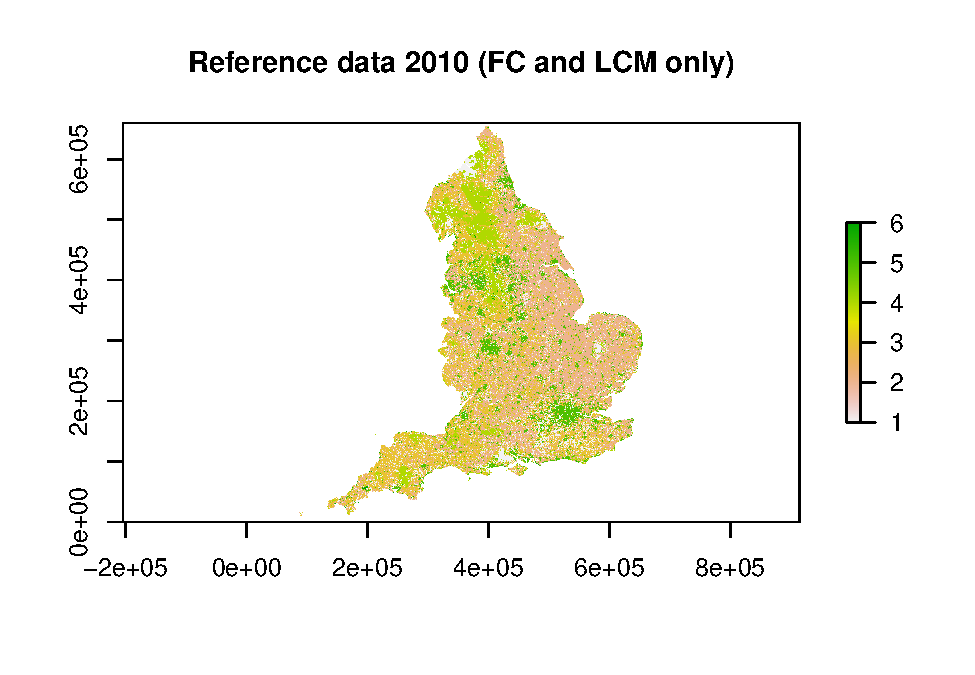
\includegraphics[width=0.5\linewidth]{bias1_files/figure-latex/unnamed-chunk-1-2}
The table below shows the reference data used for each data source:

\begin{tabular}{l|l}
\hline
Dataset & Reference\\
\hline
FC & IACS, LCM\\
\hline
IACS & FC, LCM\\
\hline
LCM & FC, IACS\\
\hline
LCC & FC, IACS, LCM\\
\hline
CORINE & FC, IACS, LCM\\
\hline
CROME & FC, IACS, LCM\\
\hline
\end{tabular}

Each data source was tested against its appropriate reference data according to the table above. The resulting 36*36 confusion matrix quantifies the correspondence between the data sets, in terms of their agreement over the area of each land use changing to every other land use. The diagonal identifies the area of land-use change that was identified to occur in both the reference and test data sets. The unchanging land on the diagonal can be disregarded as not relevant here.

\hypertarget{false-positive-rates}{%
\subsection{False positive rates}\label{false-positive-rates}}

The false positive rate was calculated as:

\(F_{Pij}\) = (\(\beta_{test,ij}\) - \(\beta_{ref,ij}\))/ \(\beta_{test,ij}\)

where \(\beta_{test,ij}\) is the observed area of land changing from use \(i\) to \(j\) in the test dataset and \(\beta_{ref,ij}\) the corresponding value in the reference dataset.

\hypertarget{false-negative-rates}{%
\subsection{False negative rates}\label{false-negative-rates}}

The false negative rate, the rate of failing to observe land-use change from \(i\) to \(j\) in the test dataset compared to the reference dataset, was calculated as:

\(F_{Nij}\) = (\(\beta_{ref,ij}\) - \(\beta_{ref,test,ij}\))/ (\(A\) - \(\beta_{test,ij}\))

where \(\beta_{ref,test,ij}\) is the area of land changing from \(i\) to \(j\) identified in both the reference and test data sets, and \(A\) is the total area of England. The denominator is thus the total land area where false negatives could occur.

\hypertarget{results-1}{%
\section{Results}\label{results-1}}

Here we use CORINE as an example showing the false positive and negative rates calculated between the data source and the reference dataset between 2006 and 2018 (most recent years available for comparison). The data shows the trend across all of the data-sources: very high false positive rates, with slightly lower false positive rates for the land-use change between crop and grassland. False negative rates were much lower, but are expressed on a very different basis, and not directly comparable. The matrices below show the false positive/negative rate for each land-use change between the first year (row) and the second year (column).

False positive rates for CORINE between 2006 and 2018:

\begin{tabular}{l|l|l|l|l|l|l}
\hline
  & woods & crops & grass & rough & urban & other\\
\hline
woods &  & 1 & 0.992 & 1 & 1 & 0\\
\hline
crops & 0.977 &  & 0.928 & 0.949 & 0.994 & 1\\
\hline
grass & 0.951 & 0.767 &  & 0.996 & 0.991 & 1\\
\hline
rough & 1 & 1 & 1 &  & 1 & 1\\
\hline
urban & 1 & 1 & 0.985 & 1 &  & 1\\
\hline
other & 0 & 1 & 1 & 1 & 0 & \\
\hline
\end{tabular}

False negative rates for CORINE between 2006 and 2018:

\begin{tabular}{l|l|l|l|l|l|l}
\hline
  & woods & crops & grass & rough & urban & other\\
\hline
woods &  & 0 & 0.001 & 0 & 0 & 0\\
\hline
crops & 0.004 &  & 0.038 & 0.001 & 0 & 0\\
\hline
grass & 0.01 & 0.053 &  & 0.009 & 0.001 & 0\\
\hline
rough & 0 & 0 & 0.011 &  & 0 & 0\\
\hline
urban & 0.004 & 0 & 0.002 & 0.003 &  & 0\\
\hline
other & 0 & 0 & 0 & 0 & 0 & \\
\hline
\end{tabular}

The following graphs show the false positive and false negative rates for each data source, with the grid of graphs showing the land use type in the first year and colour showing the land use in the second year.

False positive rates:
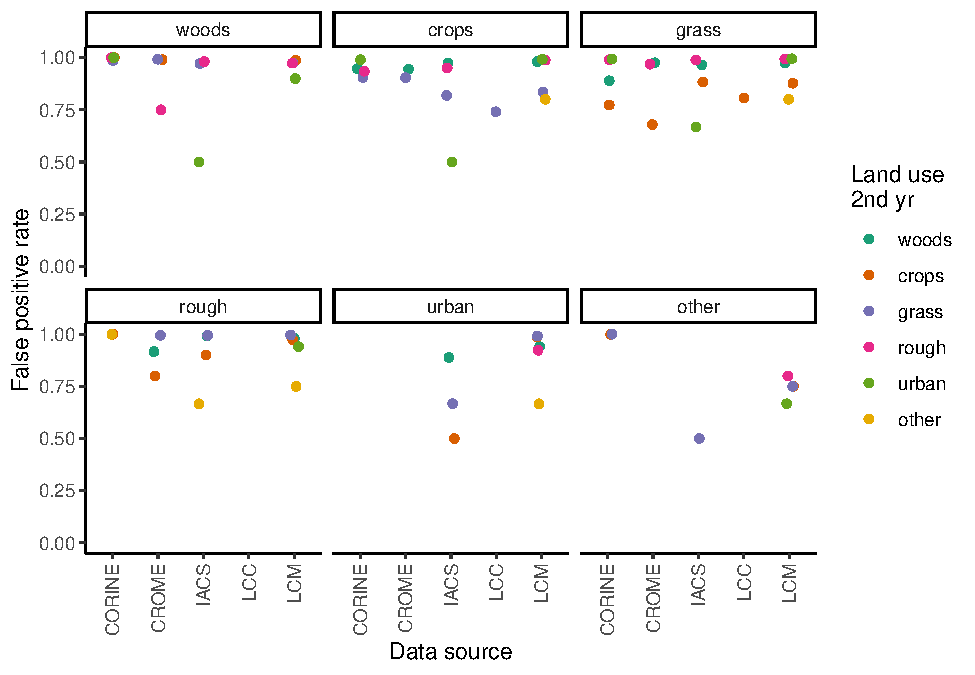
\includegraphics{bias1_files/figure-latex/graphing false positives-1.pdf}

False negative rates:
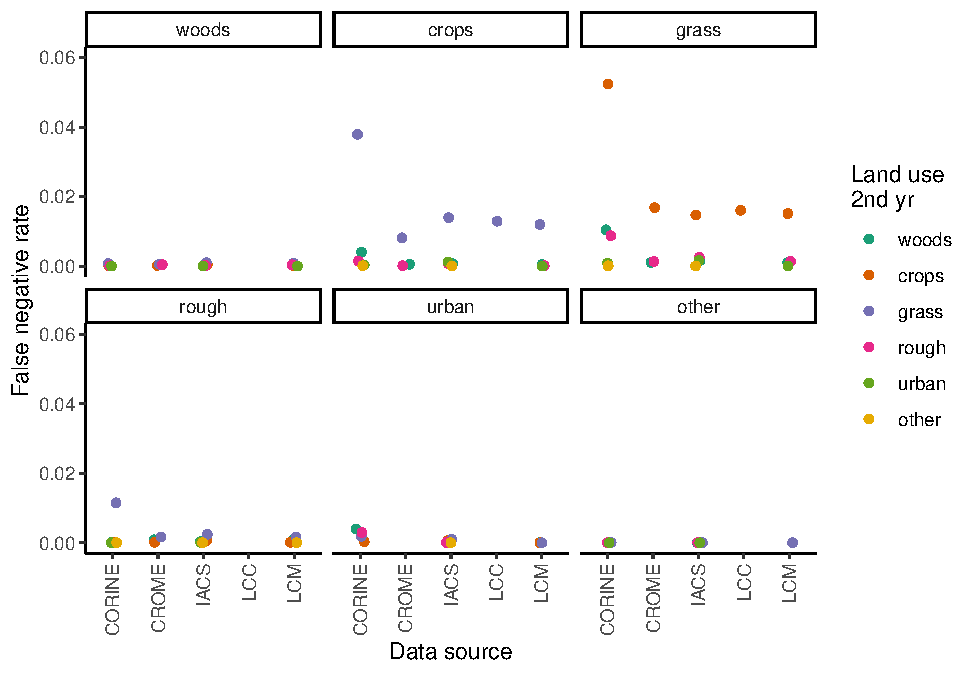
\includegraphics{bias1_files/figure-latex/graphing false negatives-1.pdf}

\hypertarget{data-source-specific-false-positive-and-false-negative-rates}{%
\subsection{Data-source-specific false positive and false negative rates}\label{data-source-specific-false-positive-and-false-negative-rates}}

Based on the relatively low variability in false positive rates identified for many of the land-use change classes, we chose to summarise false positive rates at the data-source level rather than land-use level. Data-set level false positive rates were calculated as an average of the land-use level false positive rate, weighted by area of each land-use change.

This gave the following outputs which can be incorporated into the data assimilation method:

\begin{tabular}{l|r|r}
\hline
Data source & Fn & Fp\\
\hline
FC & 0.0020230 & NA\\
\hline
LCM & 0.0013481 & 0.8711168\\
\hline
CORINE & 0.0060332 & 0.9029868\\
\hline
LCC & 0.0012670 & 0.6737150\\
\hline
IACS & 0.0020691 & 0.7997226\\
\hline
CROME & 0.0012571 & 0.9329713\\
\hline
\end{tabular}

\hypertarget{updating-b-d-g-and-l}{%
\subsection{\texorpdfstring{Updating \(B, D, G\) and \(L\)}{Updating B, D, G and L}}\label{updating-b-d-g-and-l}}

To examine the effect of these systematic biases on the observations, we can recalculate the \(B\) transition matrix. An example is provided below for IACS from 2005 to 2019:

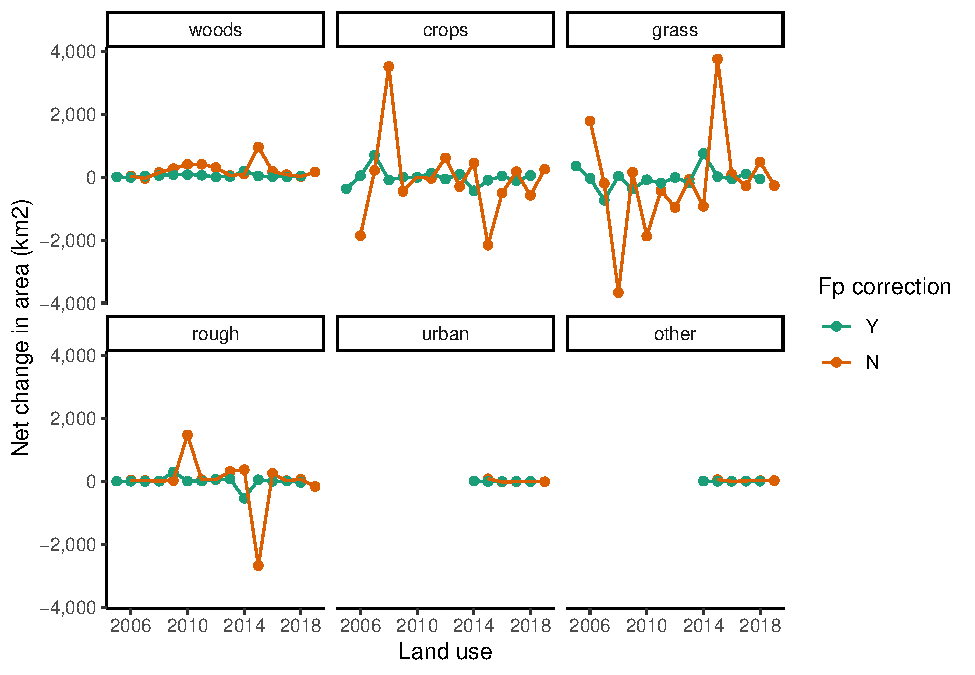
\includegraphics{bias1_files/figure-latex/updating BLAG-1.pdf}

\hypertarget{conclusions}{%
\section{Conclusions}\label{conclusions}}

\begin{itemize}
\tightlist
\item
  We can represent data source-specific systematic uncertainty by estimating appropriate false positive and false negative rates for each data source, and adding these terms to the likelihood function.
\item
  Again, the most fundamental problem is the absence of any data which we regard as ``true''. There is no immediate solution to this, and a pragmatic approach is to define a reference data set, with more or less subjectivity/expert judgement, and principles from cross-validation.
\item
  False positive rates appear to be very high, but are consistently so across most of the land-use categories. With this in mind, we use data-set level \(Fp\) and \(Fn\) values rather than land-use level values.
\end{itemize}

\begin{verbatim}
## Computation time (excl. render): 57.24 sec elapsed
\end{verbatim}

\hypertarget{assessing-systematic-errors-in-estimates-of-land-use-change-sensitivity-to-survey-interval-length}{%
\chapter{Assessing systematic errors in estimates of land-use change: sensitivity to survey-interval length}\label{assessing-systematic-errors-in-estimates-of-land-use-change-sensitivity-to-survey-interval-length}}

\hypertarget{introduction-3}{%
\section{Introduction}\label{introduction-3}}

The spatial datasets used in the data assimilation for Land Use Tracking will contain systematic errors, related to falsely detecting land-use change when it has not occurred, and missing true land-use change when it does occur.
To characterise uncertainties in the data, we want to quantify these false positive and false negative detection rates.
These have previously been estimated by comparison with a reference dataset, and thereby judging where the observed changes in a given data set are correctly identified or not. However, this depends on the validity of the reference dataset as a standard for comparison, and we know that the reference data set is imperfect. Here we use an alternative method that assesses these error rates by analysing the apparent rate of land-use change as a function of the time interval between surveys. In the absence of systematic errors, no relationship with survey-interval length would be expected, and any apparent sensitivity can be used to infer the error rates.

The observed area changing from one land-use type \(i\) to another \(j\) between two surveys, \(\beta_{ij}^{\mathrm{obs}}\) (in km\(^2\) yr\(^{-1}\)), will be made up of the true rate of change, \(\beta_{ij}\) and systematic and random error terms. Systematic errors comprise false postive (\(F^P\)) and false negative rates (\(F^N\)). Together with the random error term \(\epsilon_{ij}\), we can express our expectation for the observations to be:

\begin{equation} \label{eq:beta_errors}
\beta_{ij}^{\mathrm{obs}} = \beta_{ij} + (F_{ij}^P - F_{ij}^N) + \epsilon_{ij}
\end{equation}

As a broad approximation, we can assume that the true rate of land-use change, and the error rates, are approximately constant in time. With short intervals between surveys, there will therefore be proportionately less true change, but the magnitude of the errors will be the same. Conversely, with long intervals between surveys, the magnitude of the errors will still be the same, but there will be proportionately more true change.
As the time difference between surveys increases, the observed rate will tend towards an asymptote, equal to the true mean rate of land-use change, \(\overline{\beta_{ij}}\), as the random error term \(\epsilon_{ij}\) has a mean of zero.
We can therefore examine the apparent rate of land-use change as a function of the time interval between surveys, and infer the error rates from this relationship.
It is not possible to explicitly separate \(F^{P}\) and \(F^{N}\) in this analysis, only their net effect \(F^{\mathrm{net}} = F^{P} - F^{N}\), although the shape of curve indicates which is larger in the data. If \(F^{P}\) and \(F^{N}\) were zero, or exactly balancing each other, the data would show a flat line in the figures below. For the datasets we are testing here, in all cases it appears that false positives are the major source of error.

This method is potentially superior to estimating error rates by comparison with a reference dataset, as it does not require reliable ground-truth data, and only uses intrinsic properties of the observations. As a down-side, the error rates calculated apply to ongoing directional change, and any rotational change is effectively included in the error term. However, we note that this is only really an issue with crop-grass transitions (and v.v.), and we estimate, this affects around \textasciitilde7 \% of the grassland area (assuming that half the area of grassland \textless{} 5 years old has a rotation length shorter than the observation period). The method also assumes that the true mean rate of land use change has not changed systematically over the observation period.

\hypertarget{methods-2}{%
\section{Methods}\label{methods-2}}

\begin{itemize}
\tightlist
\item
  Calculate beta matrices for land-use change with all possible permutations of between-survey intervals available with each data source
\item
  Plot the relationship between time-interval length (\(\Delta\)) and the apparent rate of land-use change
\item
  For each term in the \(\beta\) matrix, we fit an exponential model to the data using nonlinear least squares:
\end{itemize}

\begin{equation} \label{eq:asymptote}
\beta_{ij\Delta}^{obs} = \overline{\beta_{ij}} + (A_0 - \overline{\beta_{ij}}) \mathrm{exp(-exp}(k) \Delta)
\end{equation}

where \(\overline{\beta_{ij}}\) is the asymptotic value, equal to the long-term mean rate of land-use change, \(A_0\) is the intercept at \(\Delta = 0\), and \(k\) is the natural logarithm of the rate constant.

From the fitted model, we obtain estimates of \(\overline{\beta_{ij}}\) and the value of \(\beta_{ij\Delta}^{obs}\) as a function of the time interval \(\Delta\).
We can then estimate the mean net error rate for a given time interval from the fitted curve, expressing this as a fraction of the observed rate:

\begin{equation} \label{eq:Fnet_errors}
F_{ij\Delta}^\mathrm{net} = (\beta_{ij\Delta}^{\mathrm{obs}} - \overline{\beta_{ij}}) / \beta_{ij\Delta}^{\mathrm{obs}}
\end{equation}

\hypertarget{results-2}{%
\section{Results}\label{results-2}}

In almost all cases, we see very strong sensitivity to survey-interval length, with much higher apparent rates of change observed at short interval lengths. This implies the observations are dominated by false positives; no relationship would be expected in the absence of such errors. Similar trends are seen in all the data sets examined here.

\hypertarget{iacs}{%
\subsection{IACS:}\label{iacs}}

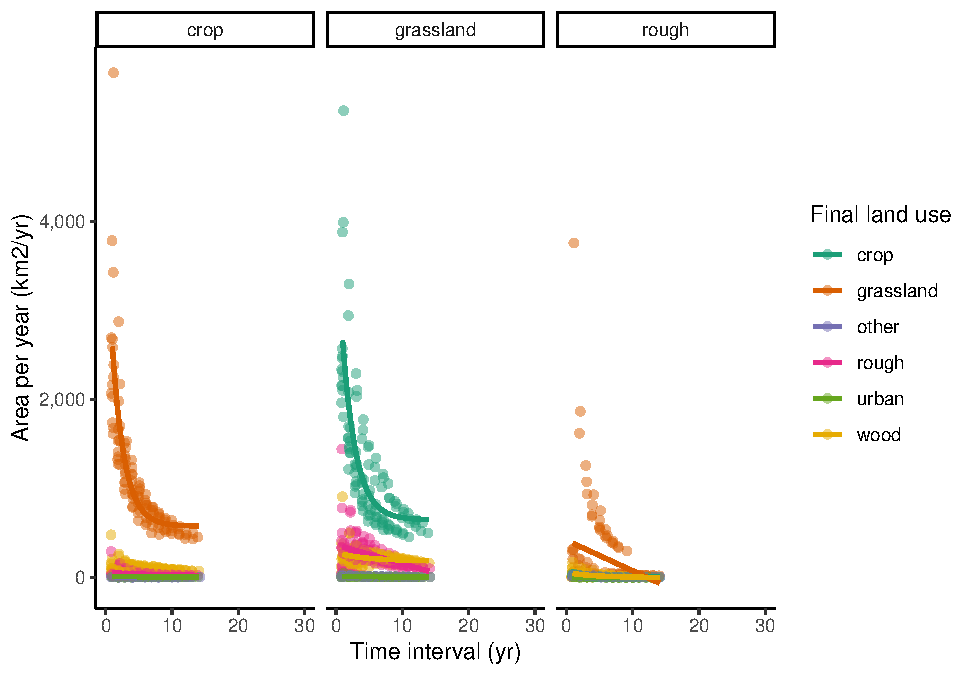
\includegraphics{time_interval_analysis_files/figure-latex/test-1.pdf} 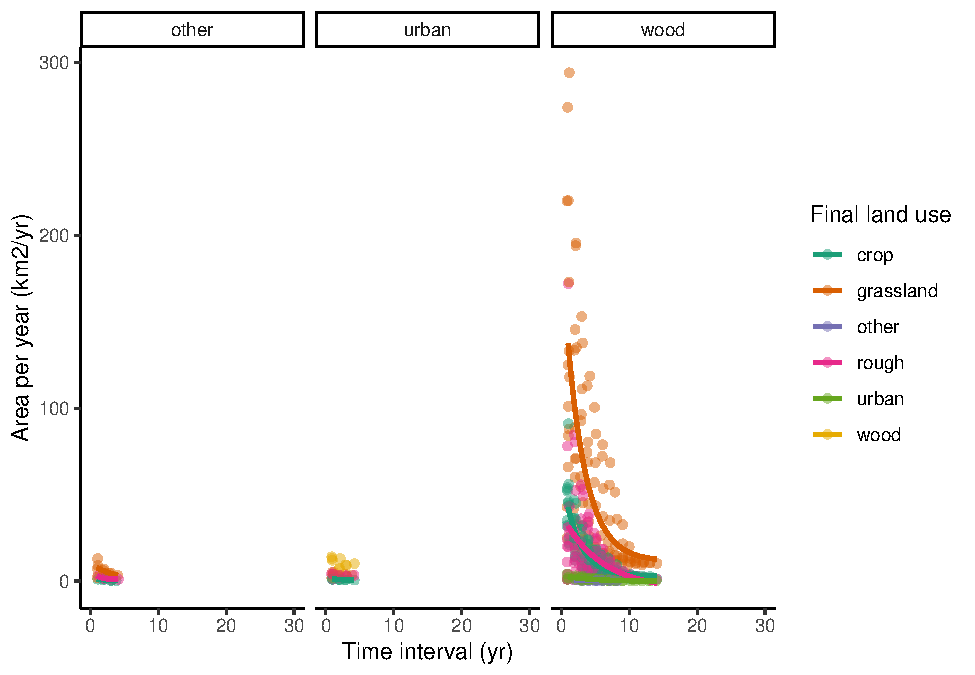
\includegraphics{time_interval_analysis_files/figure-latex/test-2.pdf}

\hypertarget{lcm}{%
\subsection{LCM}\label{lcm}}

LCM has the greatest number of datasets to apply this method to with 10 surveys conducted across 29 years. This enables comparison between surveys that give 23 time intervals.

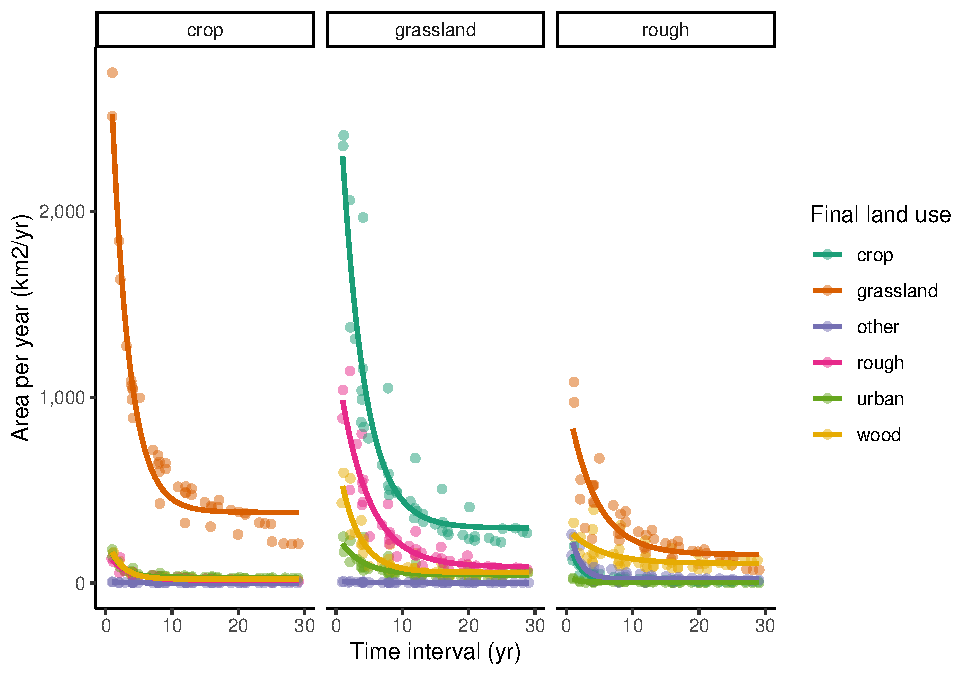
\includegraphics{time_interval_analysis_files/figure-latex/lcm-1.pdf} 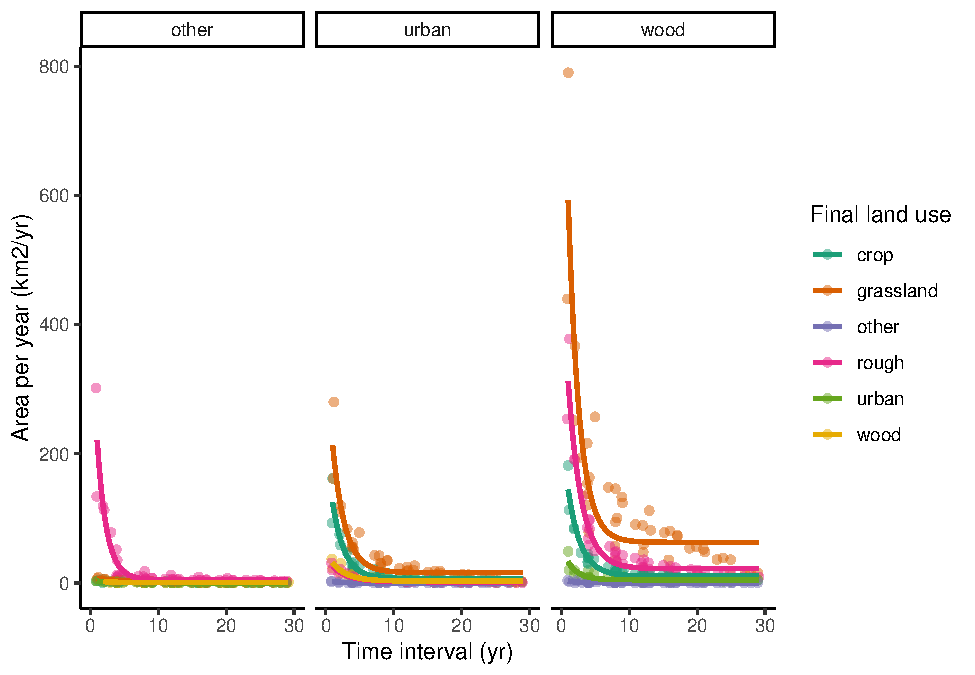
\includegraphics{time_interval_analysis_files/figure-latex/lcm-2.pdf}

\hypertarget{lcc}{%
\subsection{LCC:}\label{lcc}}

LCC only includes crop and grassland land use change so there are less data to test.

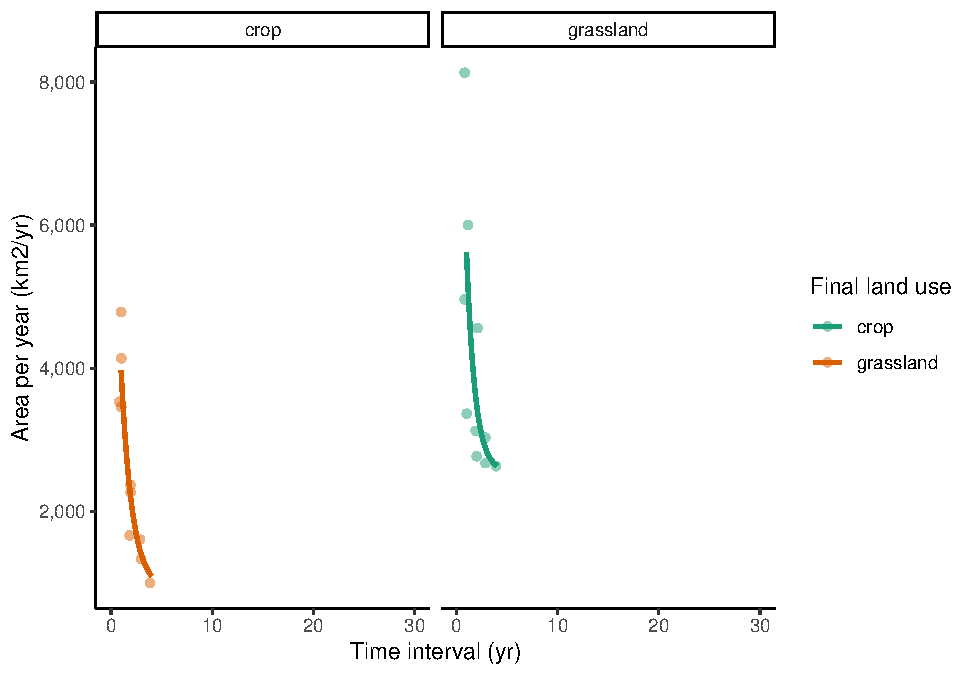
\includegraphics{time_interval_analysis_files/figure-latex/lcc-1.pdf}

\hypertarget{crome}{%
\subsection{CROME:}\label{crome}}

Both CROME and CORINE have few surveys meaning estimating a fit to this data is difficult:

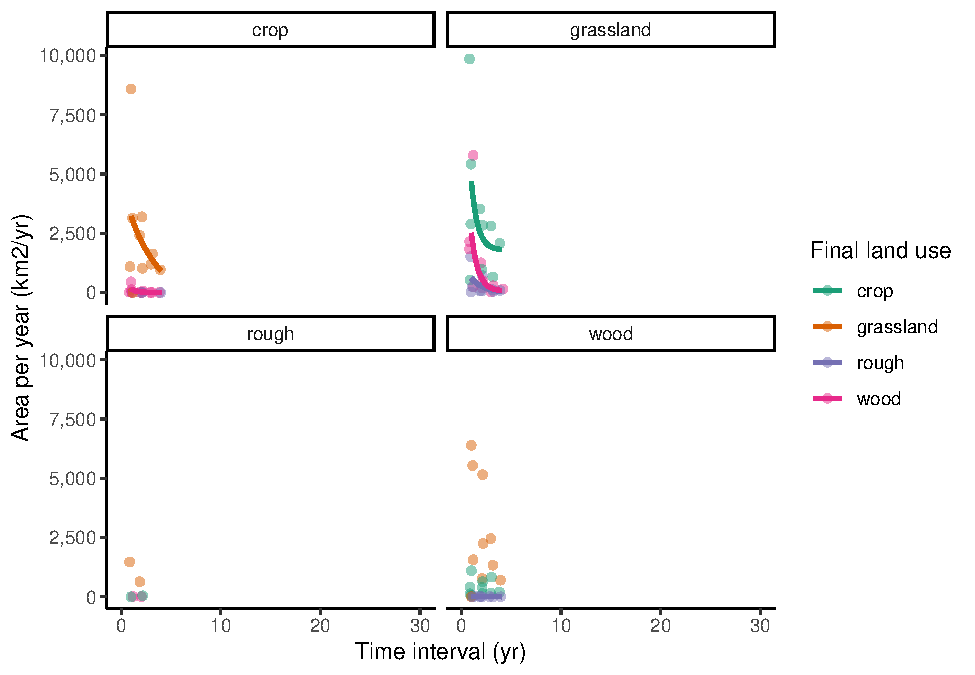
\includegraphics{time_interval_analysis_files/figure-latex/crome-1.pdf}

\hypertarget{corine}{%
\subsection{CORINE:}\label{corine}}

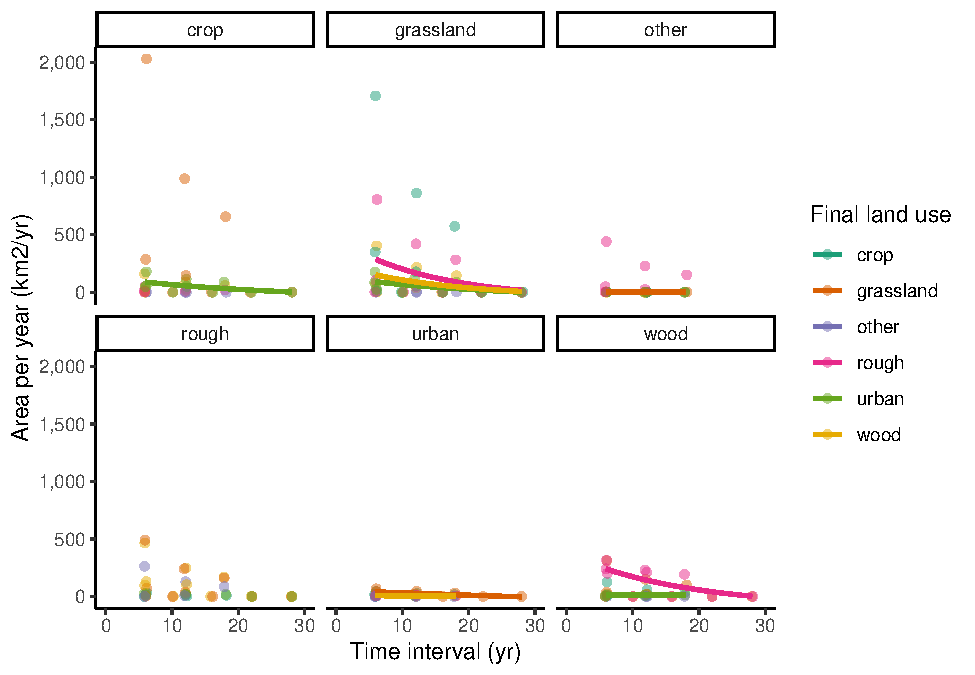
\includegraphics{time_interval_analysis_files/figure-latex/corine-1.pdf}

\hypertarget{summary-table}{%
\subsection{Summary Table}\label{summary-table}}

The table below shows the error rate for all of the different land use change categories for each of the different data sets. These are calculated for the typical time interval in each of the different data sources.

\begin{tabular}{l|r|r|r|r|r}
\hline
luc & IACS & LCM & LCC & CORINE & CROME\\
\hline
crop\_grassland & 0.78 & 0.85 & 0.77 & NA & NA\\
\hline
crop\_other & 0.82 & 0.87 & NA & NA & NA\\
\hline
crop\_rough & 0.68 & 0.87 & NA & NA & NA\\
\hline
crop\_urban & 0.96 & 0.80 & NA & NA & NA\\
\hline
grassland\_crop & 0.76 & 0.87 & 0.55 & NA & 0.62\\
\hline
grassland\_other & 0.78 & 0.84 & NA & NA & NA\\
\hline
grassland\_urban & 0.83 & 0.79 & NA & NA & NA\\
\hline
grassland\_wood & 0.28 & 0.89 & NA & NA & 0.98\\
\hline
other\_rough & 0.66 & 0.98 & NA & NA & NA\\
\hline
rough\_crop & 0.89 & 0.90 & NA & NA & NA\\
\hline
rough\_urban & 0.96 & 0.82 & NA & NA & NA\\
\hline
urban\_crop & 0.65 & 0.94 & NA & 0.87 & NA\\
\hline
wood\_crop & 0.93 & 0.93 & NA & NA & NA\\
\hline
wood\_grassland & 0.92 & 0.89 & NA & NA & NA\\
\hline
crop\_wood & NA & 0.87 & NA & NA & 0.98\\
\hline
grassland\_rough & NA & 0.91 & NA & NA & NA\\
\hline
other\_crop & NA & 0.86 & NA & 0.95 & NA\\
\hline
other\_grassland & NA & 0.83 & NA & 0.95 & NA\\
\hline
other\_urban & NA & 0.87 & NA & NA & NA\\
\hline
rough\_grassland & NA & 0.82 & NA & NA & NA\\
\hline
rough\_other & NA & 0.90 & NA & NA & NA\\
\hline
rough\_wood & NA & 0.60 & NA & NA & NA\\
\hline
urban\_grassland & NA & 0.92 & NA & NA & NA\\
\hline
urban\_other & NA & 0.93 & NA & NA & NA\\
\hline
urban\_rough & NA & 0.93 & NA & NA & NA\\
\hline
urban\_wood & NA & 0.90 & NA & 0.90 & NA\\
\hline
wood\_other & NA & 0.91 & NA & NA & NA\\
\hline
wood\_rough & NA & 0.93 & NA & NA & NA\\
\hline
wood\_urban & NA & 0.85 & NA & 0.73 & NA\\
\hline
\end{tabular}

The figure below shows the same data plotted for all data sources.

\includegraphics{time_interval_analysis_files/figure-latex/unnamed-chunk-1-1.pdf}

\hypertarget{discussion-and-conclusions}{%
\section{Discussion and Conclusions}\label{discussion-and-conclusions}}

The error rates we obtain from this method are similar to those derived from comparison with the reference data set. The net positive error rates are generally in the range 80-98 \%; that is, 80-98 \% of the ostensibly observed land-use change did not actually occur. Almost all other values in the range 50-80 \% (with only one exception less than this).
The conclusion from this is that these observations are extremely over-sensitive, and for whatever reason, differences in imagery (or survey data in the case of IACS) at different times is being recorded as land-use change when none has occurred.\\
This makes it challenging to extract useful information from these data.
However, if we believe the error rates to be consistent, we can specify and correct for these errors in the data assimilation procedure, as described previously.
Land-use-change-specific rates can be estimated from this analysis, to capture the variability in errors between different land-use conversions. However, the error rates are broadly similar, and a single value per data source could justifiably be used.
To explore this further, confidence intervals can also be calculated for the error rates in the table above, using the standard errors in the parameters from the exponential model fit.
If the errors are not consistent in time, and given their magnitude of 80-98 \%, an alternative conclusion would be that these observations are not yet reliable enough to include in the inventory procedure for tracking land-use change.

\hypertarget{estimating-false-positive-rates-in-detection-of-land-use-change-based-on-classification-accuracy}{%
\chapter{Estimating false-positive rates in detection of land-use change based on classification accuracy}\label{estimating-false-positive-rates-in-detection-of-land-use-change-based-on-classification-accuracy}}

\hypertarget{introduction-4}{%
\section{Introduction}\label{introduction-4}}

In the ``Tracking Land-Use Change'' project, several data sources provide a time series of maps of land use. An obvious approach is to estimate land-use change as the difference between these maps over time. However, any error in land classification will also be included in the estimate of land-use change, so it is important to quantify these errors properly and note how they propagate.
Here, we show the calculations which propagate the error in classification through to its resulting effect on the estimate of land-use change.

\hypertarget{methods-3}{%
\section{Methods}\label{methods-3}}

The accuracy of land-use maps is usually estimated by comparison with some reference data set. We can then calculate confusion matrices and metrics of overall agreement, of which there are several. Common choices are overall accuracy (\(\alpha\), the fraction of locations where estimated land use agrees with the reference data set) and the \(\kappa\) statistic, which corrects for the probability of chance agreement. \(\kappa\) therefore gives a more robust measure, typically 5-20 \% lower than simple percentage agreement. The probability of misclassification can be estimated simply as 1 - \(\alpha\) or more stringently as 1 - \(\kappa\). For maps at times \(t_1\) and \(t_2\), the probabilities of misclassification are denoted \(p_1\) and \(p_2\). Estimating land-use change involves calculating the difference between maps, and the errors are additive in the result. The probability of estimating erroneous land-use change because of misclassification in a pair of maps can be written as

\begin{equation} \label{eq:probmis}
  p_{1 \cup 2} = p_1 + p_2 - p_{1 \cap 2}.
\end{equation}

That is, the probability of error is the union of two events (misclassification occurring at time 1 or at time 2, minus their intersection \(p_{1 \cap 2}\), which is the probability of misclassification at both time 1 and time 2, which would otherwise be double-counted. \(p_{1 \cap 2}\) can be estimated as \(p_1 p_2\) assuming that the errors leading to misclassification at times 1 and 2 are independent of each other.
In practice, our estimates of the probabilities of misclassification at times 1 and 2 are usually the same (\(p_1 \simeq p_2\)), so this simplifies to:

\begin{equation} \label{eq:probmis2}
  p_{1 \cup 2} = 2 p_1 - p_1^2.
\end{equation}

\hypertarget{results-3}{%
\section{Results}\label{results-3}}

Estimates of \(\alpha\) and \(\kappa\) from some of the data sets used in the LUC Tracking project are shown in the table below.

\begin{tabular}{l|r|r}
\hline
Data source & $\alpha$ & $\kappa$\\
\hline
Corine & 0.80 & 0.64\\
\hline
LCC & 0.91 & 0.82\\
\hline
LCM & 0.88 & NA\\
\hline
\end{tabular}

For the purposes of the examples below, we use the value of 0.88, the overall accuracy of the LCM, as a relatively optimistic metric.
The value of \(p_1 \simeq p_2\) is 1 - \(\alpha\), and therefore = 0.12.

Using this value in Equation \ref{eq:probmis2} yields a probability of estimating erroneous land-use change because of misclassification of 0.226.
Because this probability applies at every location on the map, multiplying by the total area yields the expected area of erroneous land-use change.
So, when comparing two UK maps which each have a classification accuracy of 88 \%, 22.6 \% of the area, around 55000 km\(^2\), will show land-use change where none actually occurs. This provides a huge amount of measurement noise when we are attempting to detect a very small signal: the expected magnitude of actual land use change in the UK is of the order of a few hundred km\(^2\), and at most a few thousand km\(^2\), based on Forestry Commission planting rates, Agricultural Census, and urban expansion data. The area of land changing use is thus less than 1 \% of the total area, and we would therefore need the probability of misclassification error to be less than this in order to accurately detect true change (meaning the accuracy needs to be \textgreater{} 99 \%).

We can extend this to calculate the false positive rates for terms in the \(\beta\) matrix and gross gains and losses, given the appropriate denominators and estimates of the true extent of land-use change. For example, the area of cropland in England is approximately 45000 km\(^2\), and the area of gross gains and losses are estimated to be in the range 300-800 km\(^2\) y\(^{-1}\) based on CS. Based on the June Agricultural Census, we might estimate these rates to be higher, perhaps reaching 1000-3000 km\(^2\) y\(^{-1}\).

Expressing the estimated true land-use change \(A_{true}\) as a fraction of the total recorded land-use change (i.e.~true + erroneous), we can calculate the relevant false positive rate, \(F_P\).

\begin{equation} \label{eq:falsepos}
  F_P = 1 - \frac{A_{true}}{A_{true} + A_{false}}
\end{equation}

If CS rates of land-use change are correct (300-800 km\(^2\) y\(^{-1}\)), the false positive rate is in the range 92.7 to 97.1 \%.

If the Agricultural Census rates of land-use change are correct (1000-3000 km\(^2\) y\(^{-1}\)), the false positive rate is in the range 77.2 to 91 \%.

Given this relationship between the classification accuracy of individual maps and the resulting false positive rates in detecting land-use change, we can examine the improvement needed to obtain false positive rates below a given level. The figure below shows the change in false positive rate with classification error (1- \(\alpha\)), using the example of cropland gains in England as above, assuming a true rate of change of 1000 km\(^2\) y\(^{-1}\).

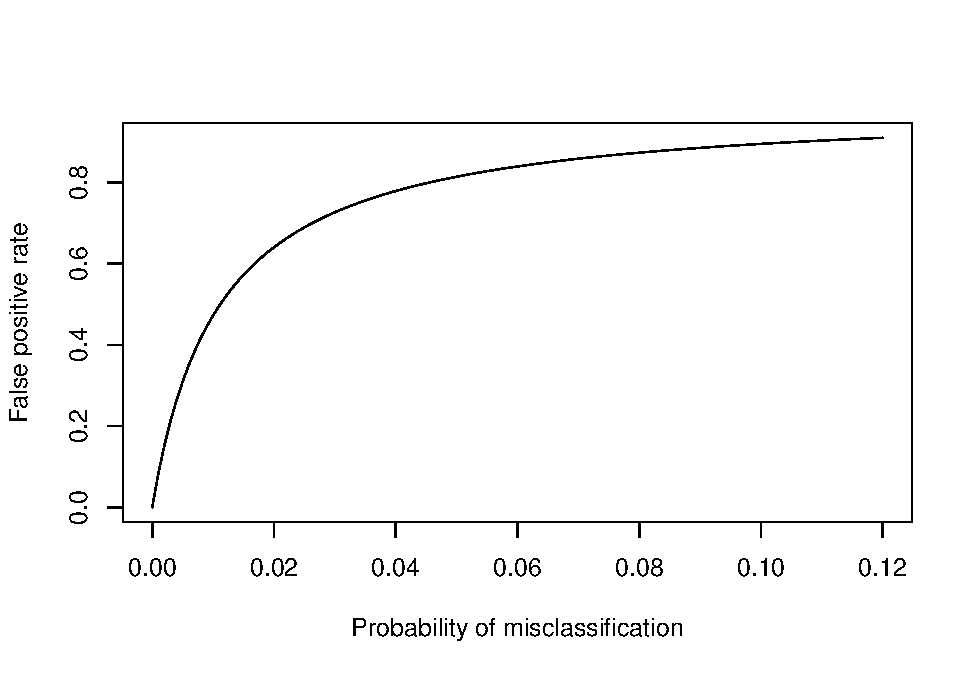
\includegraphics{fp_from_accuracy_files/figure-latex/unnamed-chunk-5-1.pdf}

The figure shows asymptotic behaviour because of the form of Equation \ref{eq:falsepos}, with a constant true area expressed with an increasing \(A_{false}\) term in the denominator. The result is that it takes a substatial decrease in misclassification (or increase in accuracy) from present values to achieve a marked increase in the false positive rate. For example, to reduce the false positive rate to 0.5 requires an accuracy of 0.988. The basic problem is that the true areas of change are very small compared to current error rates, and it would require an order of magnitude improvement in accuracy to reduce the measurement noise to a similar level to the signal we want to detect.

\hypertarget{conclusions-1}{%
\section{Conclusions}\label{conclusions-1}}

\begin{itemize}
\tightlist
\item
  Accuracy of land-use classification is in the range 0.8-0.9 in the available data sets. The corresponding probability of misclassification is 10-20 \%.
\item
  The errors in individual maps can be propagated to calculate the error in their differences i.e.~estimates of land-use change.
\item
  Error rates for land-use change propagating from misclassification will typically be greater than 20 \%. This is 1-2 orders of magnitude larger than the expected land-use change.
\item
  The probability of misclassification can be used to calculate the false positive rate of land-use change detection, and values are typically around 90 \%.
\item
  Whilst these errors are predictable and can be accounted for, directly detecting the expected land-use change rates \textless1 \% is not currently practicable.
\end{itemize}

\hypertarget{using-life-tables-in-modelling-land-use-change}{%
\chapter{Using life tables in modelling land-use change}\label{using-life-tables-in-modelling-land-use-change}}

\hypertarget{introduction-5}{%
\section{Introduction}\label{introduction-5}}

This section describes the concept of life tables in modelling land-use change. In the current procedure, we firstly estimate the \(B\) matrix each year by MCMC, then estimate where these land-use changes take place in a separate step. This second step uses static maps of likelihood for each land use. That is, for each year, we have a raster containing the likelihood of a given land-use occuring in each cell. This is based on observed data; if several data sets agree that a given cell is used for crops in a given year, there is a high likelihood of any new cropland being placed there by the algorithm (if it is not already cropland). However, these likelihood maps are static: they vary over time according to the data, but they are the same in every simulation. What this misses is the dependence of land-use change on prior history in the grid cell. There are a few cases where this is important. Most importantly, there is rotational grassland, which is used for arable crops for a number of years, before being returned to grassland on a repeating cycle. Thus, the likelihood of grassland changing to cropland is higher for a four-year old grassland than a 50-year old grassland. This phenomenon is not well captured in the current method. For forests, deforestation may be more likely to occur where the trees are at a commercially harvestable age, so the likelihood of transition is not constant, but peaks at around 40-60 years. More generally, land use shows inertia, and change is less likely where no change has happened before.

To capture such ``memory'' effects (i.e.~that the time since past land-use change affects the likelihood of current land-use change), we can use an approach borrowed from population modelling based on ``life tables''. In the population modelling context, life tables are a set of age-specific mortality rates. The same idea is referred to as survival analysis, reliability analysis, ot time-to-event analysis in various domains. Here, we are modelling the ``survival'' of land under a given continuous usage. Using the population analogy, a forest is ``born'' when a grid cell is afforested (from any other previous land use), and ``dies'' when it is deforested (converted to any other previous land use). Similarily, the same applies when areas of other land uses are created or destroyed.
We can think of this as six populations (woods, cropland, grassland, rough grazing, urban or other land uses), each of which has a specific life table. In this context, rather than mortality rates, the life table is the set of age-specific probabilities of conversion to other uses. So rather than a single dimension, each life table has six columns, for the probabilities to conversion to each of the five other land uses, plus the probability of remaining unchanged.

\hypertarget{methods-4}{%
\section{Methods}\label{methods-4}}

We established the life tables based on observed data, by counting the frequency of the length of all contiguous land uses. The land-use vectors derived from the IACS, CROME, and LCC data sets were used to do this for the six land-use classes considered here.
Within these, for each land use, we performed a cross-tabulation of the frequency of transitions to every other land use with age.
That is, taking crops as an example, we counted the occurrences of:

\begin{itemize}
\tightlist
\item
  1-year old crops changing to woods,
\item
  1-year old crops remaining as crops,
\item
  1-year old crops changing to grasslands,
\item
  1-year old crops changing to rough grazing,
\item
  \ldots{} etc., and
\item
  2-year old crops changing to woods,
\item
  2-year old crops remaining as crops,
\item
  2-year old crops changing to grasslands,
\item
  2-year old crops changing to rough grazing,
\item
  \ldots{} etc.,
\end{itemize}

and so forth, up to an age of 10 years, the longest span of continuous data available (in IACS). Normalising by total count, we can convert these frequencies to estimated probabilities.
These transition probabilities are usually denoted \(\lambda\) in the context of population modelling (probability of mortality).

\hypertarget{results-4}{%
\section{Results}\label{results-4}}

The life tables for cropland and grassland over the first ten years are shown in Figures \ref{fig:plotLFcrops} and \ref{fig:plotLFgrass}.

\begin{figure}
\centering
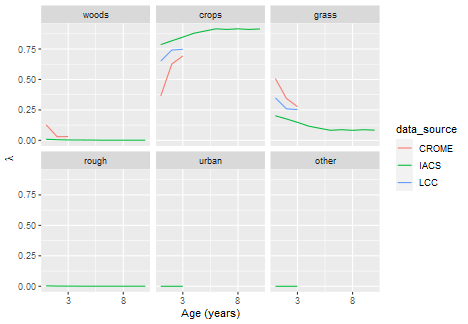
\includegraphics{lifetables_files/figure-latex/plotLFcrops-1.png}
\caption{\label{fig:plotLFcrops}The transition probability, \(\lambda\), for cropland as a function of its age (i.e.~time since previous land use). The panel labelled `crops' shows the probability of cropland remaining cropland.}
\end{figure}

\begin{figure}
\centering
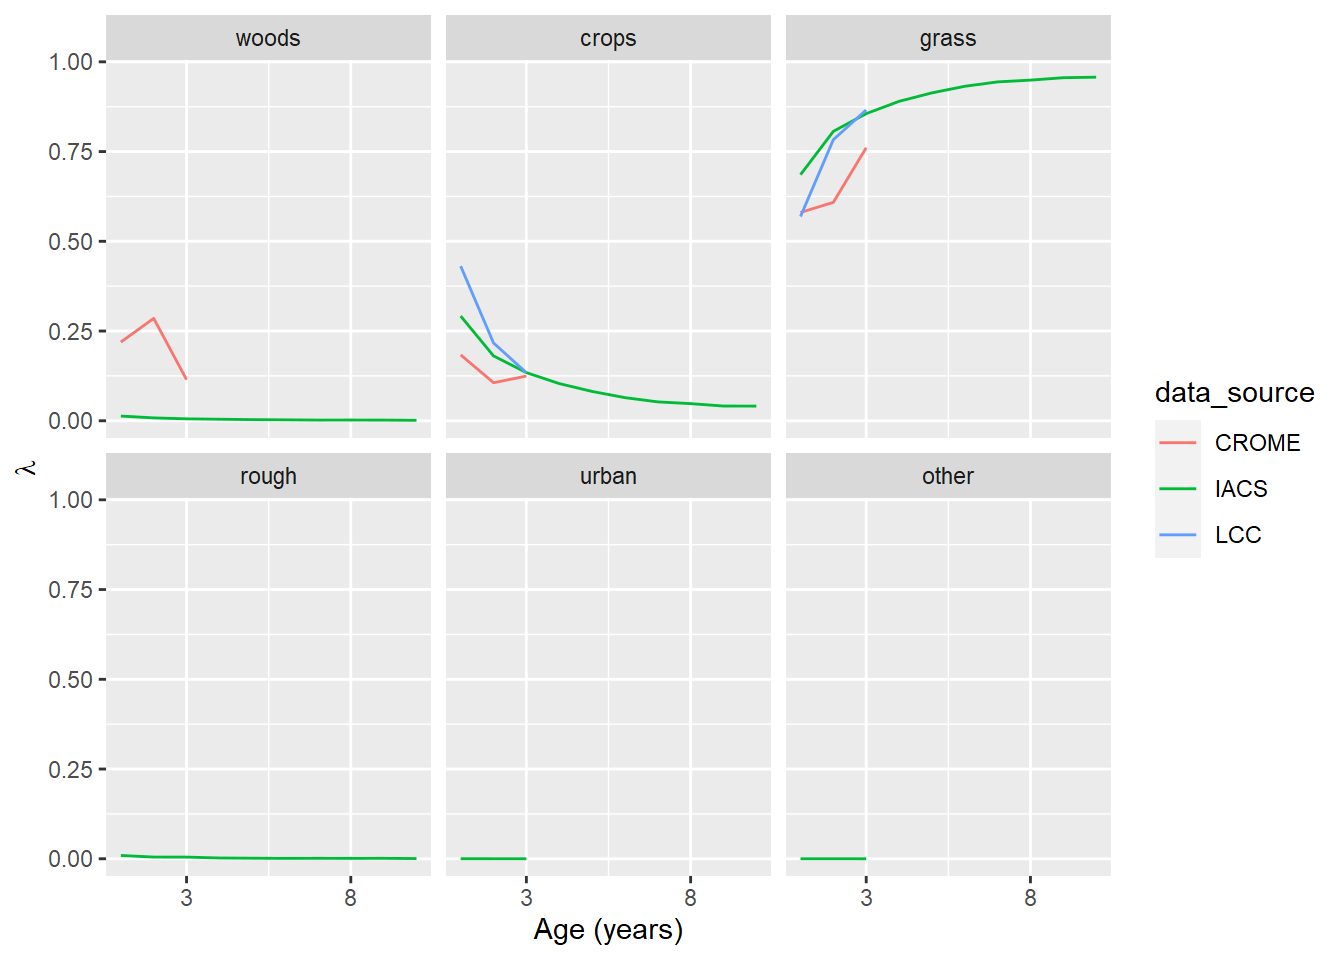
\includegraphics{lifetables_files/figure-latex/plotLFgrass-1.png}
\caption{\label{fig:plotLFgrass}The transition probability, \(\lambda\), for grassland as a function of its age (i.e.~time since previous land use). The panel labelled \emph{grass} shows the probability of grassland remaining grassland.}
\end{figure}

The three data sources show similar patterns, although initial change is generally steeper in CROME and LCC. A 10-year time span is only available in IACS, so definitive comparisons are not possible. In the case of both crops and grasslands, the probability of remaining unchanged increases asymptotically with age; the probability of changing use decreases correspondingly. The most likely transition for cropland is to grassland, and vice versa. The probability of other conversions remains low and roughly constant.

\hypertarget{discussion-1}{%
\section{Discussion}\label{discussion-1}}

The code for the data assimilation algorithm was adapted to use the life tables dynamically to calculate the likelihoods \(\mathcal{L}\) in sampling \(U\), going back in time from 2019. Previously, the likelihood calculation was done as a pre-processing step, to calculate a number of static maps, one per year.
This is now done dynamically, muliplying a spatial likelihood term \(\mathcal{L}_\mathrm{static}\) with the dynamic likelihood term \(\mathcal{L}_\mathrm{dynamic}\) (depending on the age of the current land use). Because \(\mathcal{L}_\mathrm{dynamic}\) depends only on the age (and not the whole previous history), we simply need to update a raster containing the age of each land use each year. This requires an initial estimate from which to start, and then works backwards.

Note that the absolute values in the life tables are not critical; the actual number of cells changing use is determined when we estimate the \(\beta\) matrix values.
Indeed, there are reasons not to trust the absolute values as they will include all the false positives discussed in previous sections.
It is the shape of these curves with age that is important.
Given we know how many cells are changing from (say) crop to grass each year, the table determines the relative likelihood of this occuring in new croplands versus older more established croplands.
Because the possibility of change occurs at every location every year, rotational land use is an emergent property of the simulations, at a frequency approximately the same as in the observed data.
In principle this can occur with any land use, but is only really significant with changes between crops and grass.

\begin{verbatim}
## Computation time (excl. render): 2.1 sec elapsed
\end{verbatim}

\hypertarget{results-england}{%
\chapter{Results: England}\label{results-england}}

The figures below show the results of the data assimilation procedure. All the data sets shown were used in the algorithm, but their relative random uncertainties (\(\sigma\)) determined how much influence they have on the estimates. The spatial data sets were corrected for systematic uncertainties, using the estimated net false positive rate (\(F_P\)). Having estimated the posterior distribution of the \(\beta\) matrix, we used this to simulate multiple maps of land use going back in time to 1950. The maps of the likelihood of transition to each land use established in WP-A were updated dynamically, using the life tables described in Section 5.

\begin{figure}
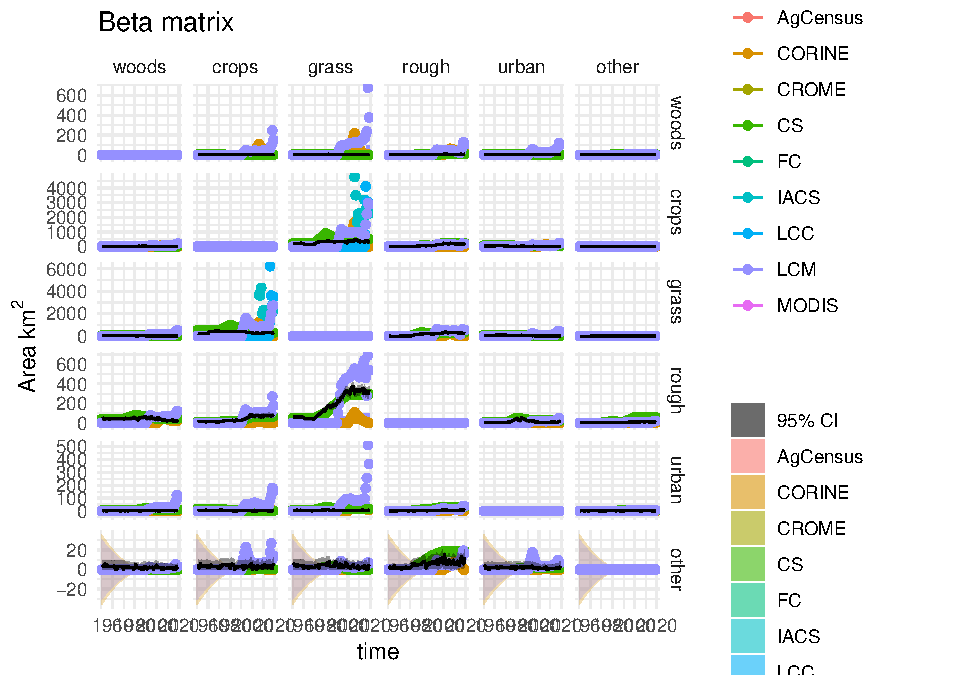
\includegraphics[width=1.3\linewidth]{Results_en_files/figure-latex/plotB-1} \caption{ Observations and posterior distribution of the transition matrix $\mathbf{B}$, representing the gross area changing from the land use in each row to the land use in each column each year from 1950 to 2020. The grey shaded band shows the 2.5 and 97.5 percentiles of the posterior distribution. The maximum *a posteriori* estimate is shown as the solid black line within this. Observations from the different data sources are shown as coloured circles. The coloured solid lines show the corrected observations after accounting for systematic uncertainties, and interpolating. The coloured bands around these lines show the random uncertainty, rescaled as $\sigma /5$ to keep with the axis scale. Because the random uncertainties and the corrections to the observations are generally very large in comparison to the actual change, scaling the axes is difficult. Note that a consistent colour scheme for the data sources is shown, but not all contribute to every figure.}\label{fig:plotB}
\end{figure}

\begin{figure}
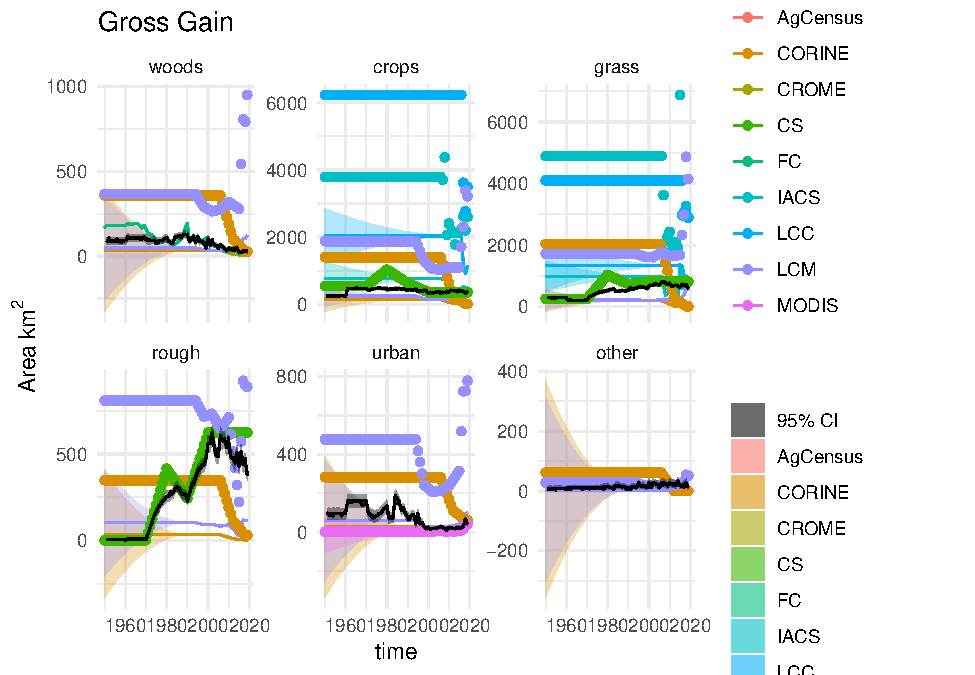
\includegraphics[width=1.3\linewidth]{Results_en_files/figure-latex/plotG-1} \caption{ Observations and posterior distribution of the gross gain in area of each land use $\mathbf{G}$ from 1950 to 2020.  The grey shaded band shows the 2.5 and 97.5 percentiles of the posterior distribution. The maximum *a posteriori* estimate is shown as the solid black line within this. Observations from the different data sources are shown as coloured circles. The coloured solid lines show the corrected observations after accounting for systematic uncertainties, and interpolating. The coloured bands around these lines show the random uncertainty, rescaled as $\sigma /5$ to keep with the axis scale. Because the random uncertainties and the corrections to the observations are generally very large in comparison to the actual change, scaling the axes is difficult. Note that a consistent colour scheme for the data sources is shown, but not all contribute to every figure.}\label{fig:plotG}
\end{figure}

\begin{figure}
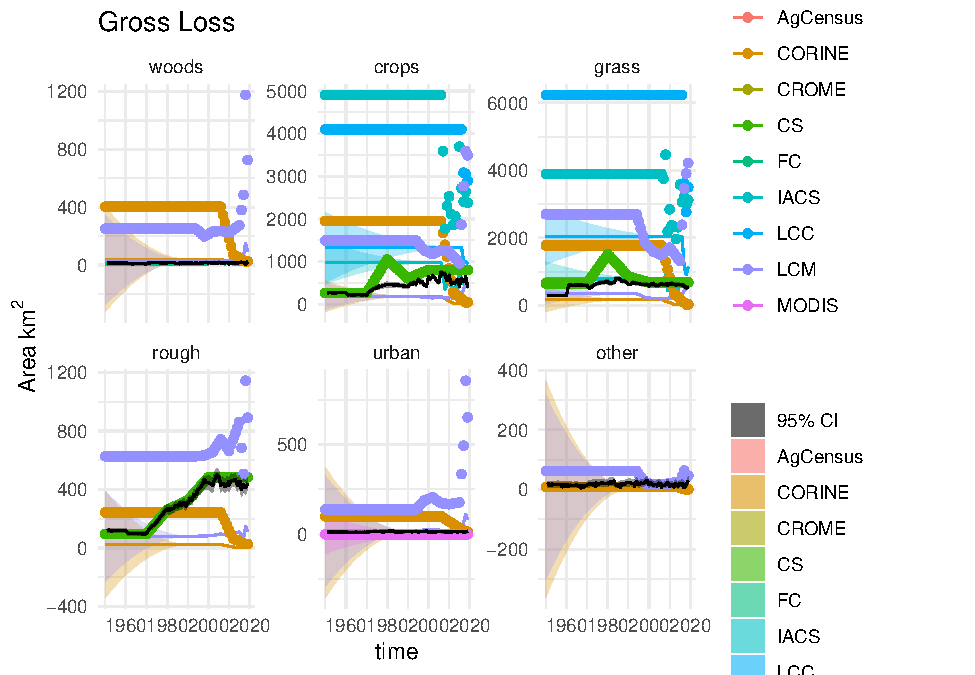
\includegraphics[width=1.3\linewidth]{Results_en_files/figure-latex/plotL-1} \caption{ Observations and posterior distribution of the gross loss of area from each land use $\mathbf{L}$ from 1950 to 2020.  The grey shaded band shows the 2.5 and 97.5 percentiles of the posterior distribution. The maximum *a posteriori* estimate is shown as the solid black line within this. Observations from the different data sources are shown as coloured circles. The coloured solid lines show the corrected observations after accounting for systematic uncertainties, and interpolating. The coloured bands around these lines show the random uncertainty, rescaled as $\sigma /5$ to keep with the axis scale. Because the random uncertainties and the corrections to the observations are generally very large in comparison to the actual change, scaling the axes is difficult. Note that a consistent colour scheme for the data sources is shown, but not all contribute to every figure.}\label{fig:plotL}
\end{figure}

\begin{figure}
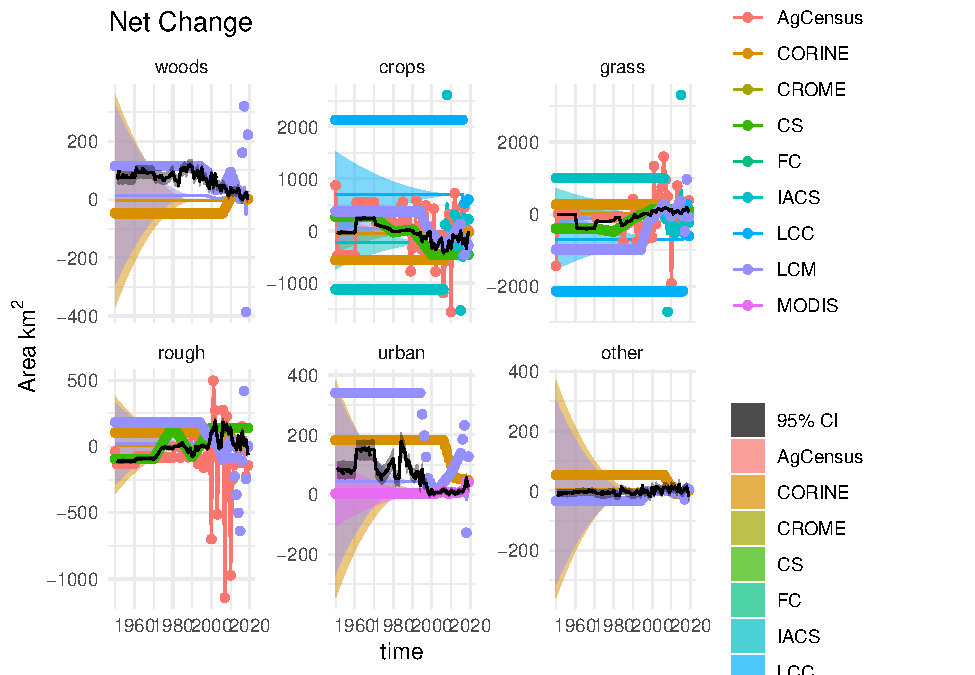
\includegraphics[width=1.3\linewidth]{Results_en_files/figure-latex/plotD-1} \caption{ Time series of the net change in area occupied by each land use ($D$) from 1950 to 2020, showing the observations and posterior distribution of estimates. The grey shaded band shows the 2.5 and 97.5 percentiles of the posterior distribution. The maximum *a posteriori* estimate is shown as the solid black line within this. Observations from the different data sources are shown as coloured circles. The coloured solid lines show the corrected observations after accounting for systematic uncertainties, and interpolating. The coloured bands around these lines show the random uncertainty, rescaled as $\sigma /5$ to keep with the axis scale. Because the random uncertainties and the corrections to the observations are generally very large in comparison to the actual change, scaling the axes is difficult. Note that a consistent colour scheme for the data sources is shown, but not all contribute to every figure.}\label{fig:plotD}
\end{figure}

\begin{figure}
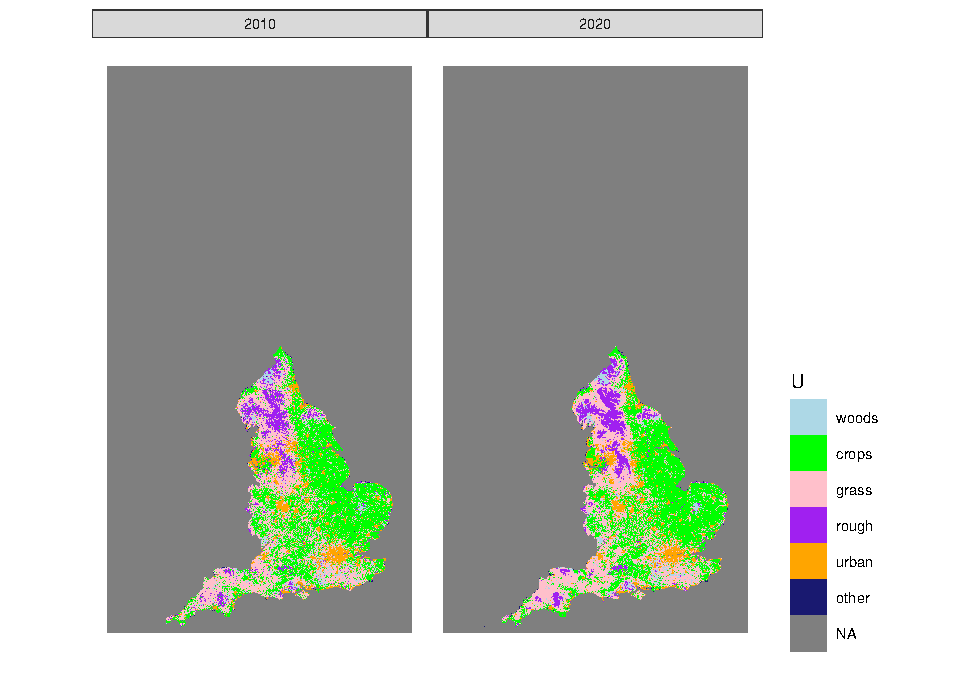
\includegraphics[width=1.3\linewidth]{Results_en_files/figure-latex/plotUt-1} \caption{Estimated state of land-use in 2010 and 2020 in one realisation of $U$ from the maximum *a posteriori* estimate of $B$.}\label{fig:plotUt}
\end{figure}

\begin{figure}
\centering
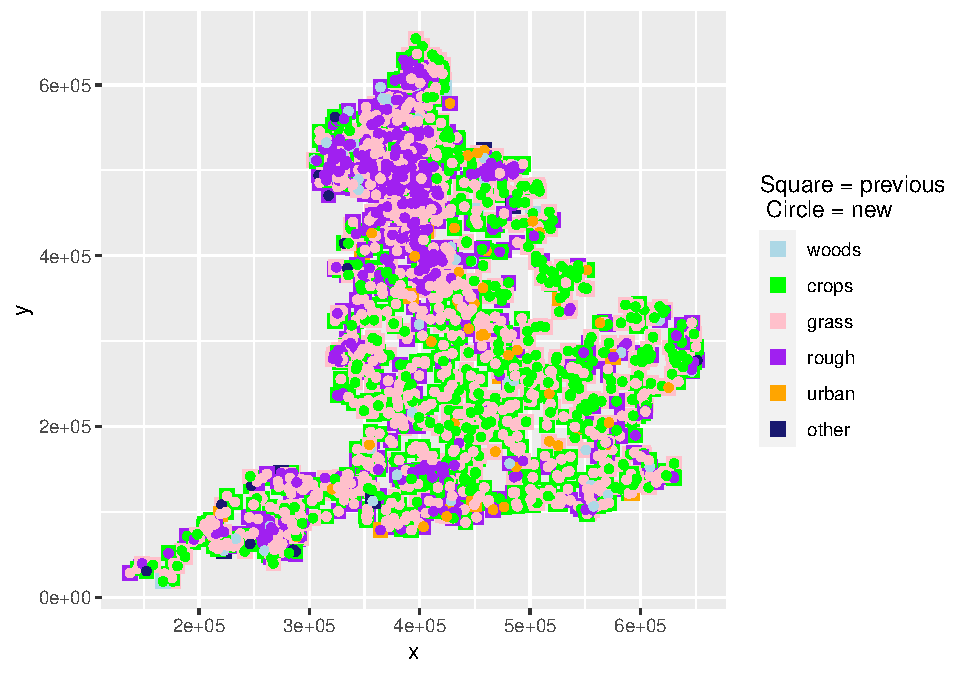
\includegraphics{Results_en_files/figure-latex/plotUd-1.pdf}
\caption{\label{fig:plotUd}The spatial distribution of land-use change between 2010 and 2020 in one realisation of \(U\) from the maximum \emph{a posteriori} estimate of \(B\). At each location where land use has changed, the use in 2010 is shown as a coloured square, and the use in 2020 is shown as a coloured circle within this}
\end{figure}

\begin{figure}
\centering
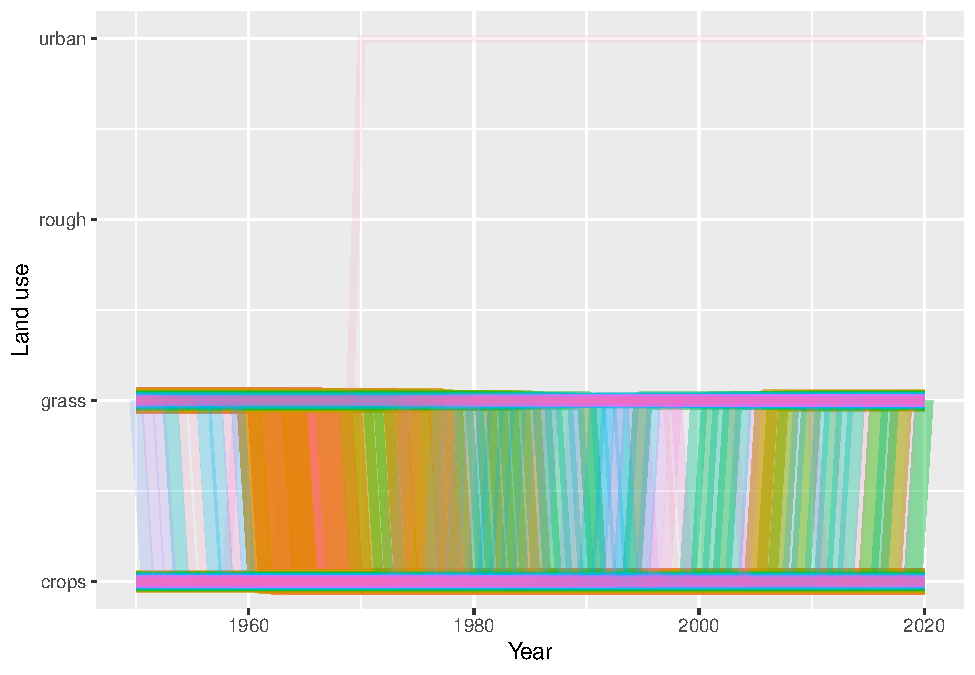
\includegraphics{Results_en_files/figure-latex/plotv1-1.pdf}
\caption{\label{fig:plotv1}Trajectories of the 100 land-use vectors in the posterior \(U\) with the largest areas (excluding the six vectors which show no change). Each vector of land use is shown in a different colour, varied arbitrarily to differentiate different vectors. Line thickness and opacity are proportional to the total area occupied by each vector, so that the dominant vectors are the most visually obvious.}
\end{figure}

\begin{figure}
\centering
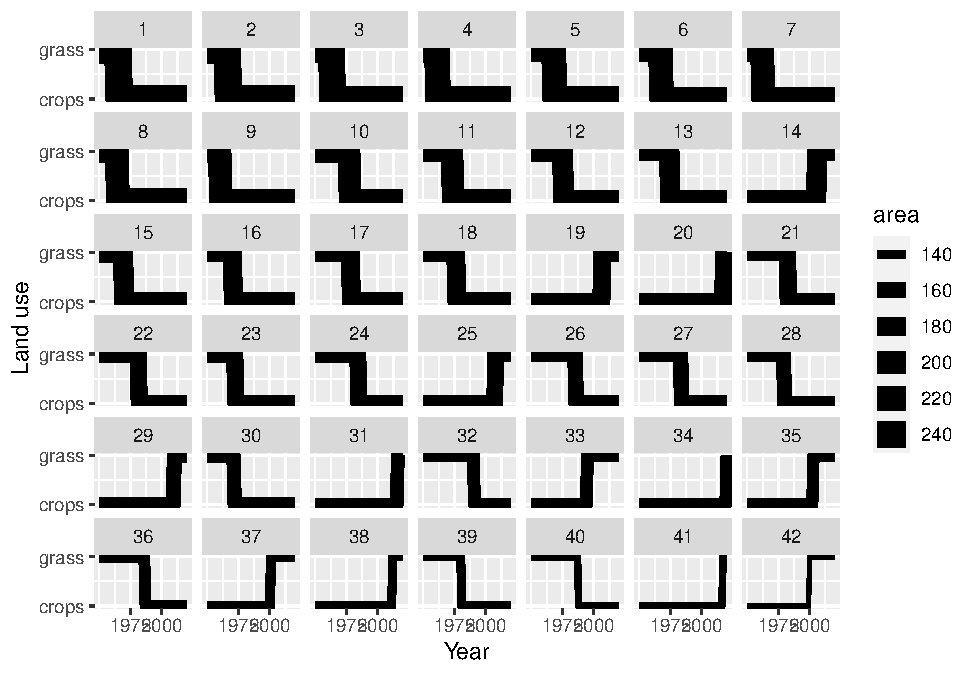
\includegraphics{Results_en_files/figure-latex/plotv2-1.pdf}
\caption{\label{fig:plotv2}Trajectories of the 42 land-use vectors in the posterior \(U\) with the largest areas (excluding the six vectors which show no change). Line thickness is proportional to the total area occupied by each vector.}
\end{figure}

\begin{figure}
\centering
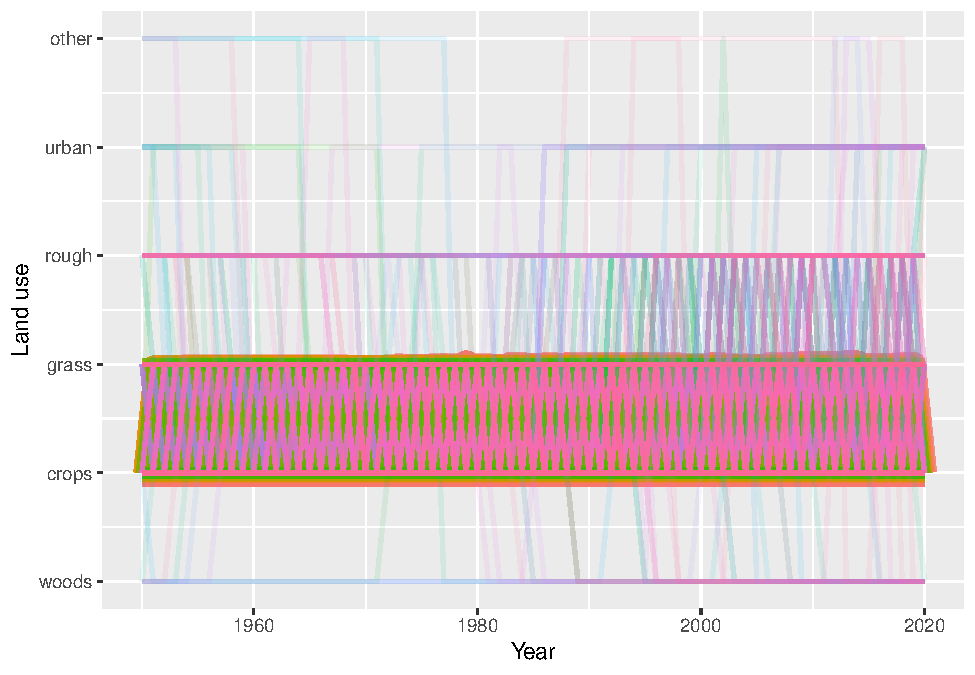
\includegraphics{Results_en_files/figure-latex/plotcgr-1.pdf}
\caption{\label{fig:plotcgr}Trajectories of the land-use vectors in the posterior \(U\) which involve rotational change between crop and grassland (i.e.~those which include either (i) transitions from crop to grass and then subsequently from grass to crop, \emph{or} (ii) transitions from grass to crop and then subsequently from crop to grass). Each vector of land use is shown in a different colour, varied arbitrarily to differentiate different vectors. Line thickness and opacity are proportional to the total area occupied by each vector, so that the dominant vectors are the most visually obvious.}
\end{figure}

\hypertarget{results-scotland}{%
\chapter{Results: Scotland}\label{results-scotland}}

The figures below show the results of the data assimilation procedure. All the data sets shown were used in the algorithm, but their relative random uncertainties (\(\sigma\)) determined how much influence they have on the estimates. The spatial data sets were corrected for systematic uncertainties, using the estimated net false positive rate (\(F_P\)). Having estimated the posterior distribution of the \(\beta\) matrix, we used this to simulate multiple maps of land use going back in time to 1950. The maps of the likelihood of transition to each land use established in WP-A were updated dynamically, using the life tables described in Section 5.

\begin{figure}
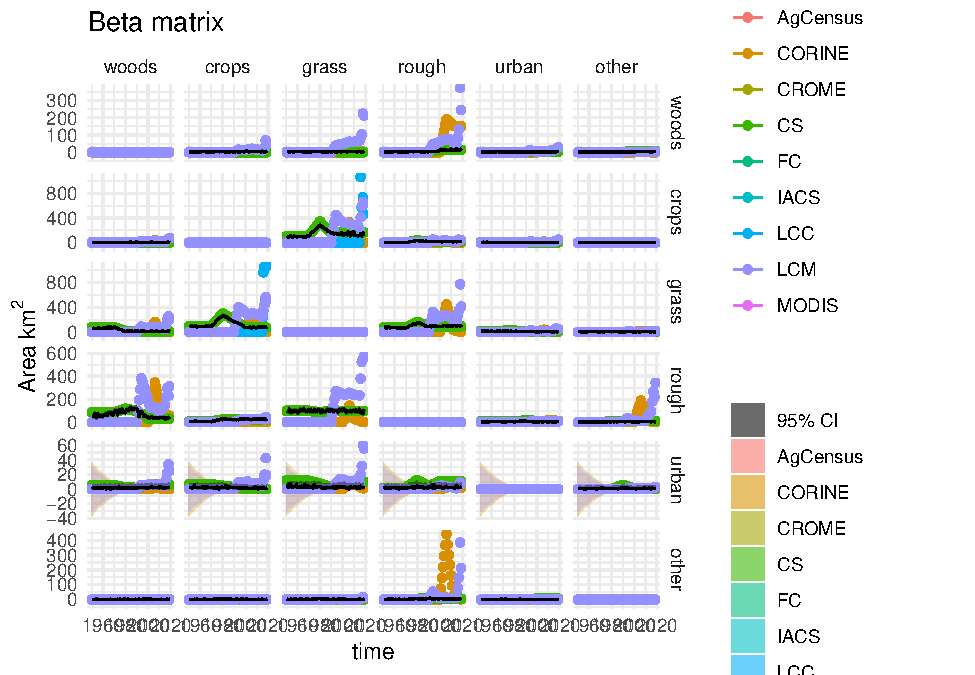
\includegraphics[width=1.3\linewidth]{Results_sc_files/figure-latex/plotB-1} \caption{ Observations and posterior distribution of the transition matrix $\mathbf{B}$, representing the gross area changing from the land use in each row to the land use in each column each year from 1950 to 2020. The grey shaded band shows the 2.5 and 97.5 percentiles of the posterior distribution. The maximum *a posteriori* estimate is shown as the solid black line within this. Observations from the different data sources are shown as coloured circles. The coloured solid lines show the corrected observations after accounting for systematic uncertainties, and interpolating. The coloured bands around these lines show the random uncertainty, rescaled as $\sigma /5$ to keep with the axis scale. Because the random uncertainties and the corrections to the observations are generally very large in comparison to the actual change, scaling the axes is difficult. Note that a consistent colour scheme for the data sources is shown, but not all contribute to every figure.}\label{fig:plotB}
\end{figure}

\begin{figure}
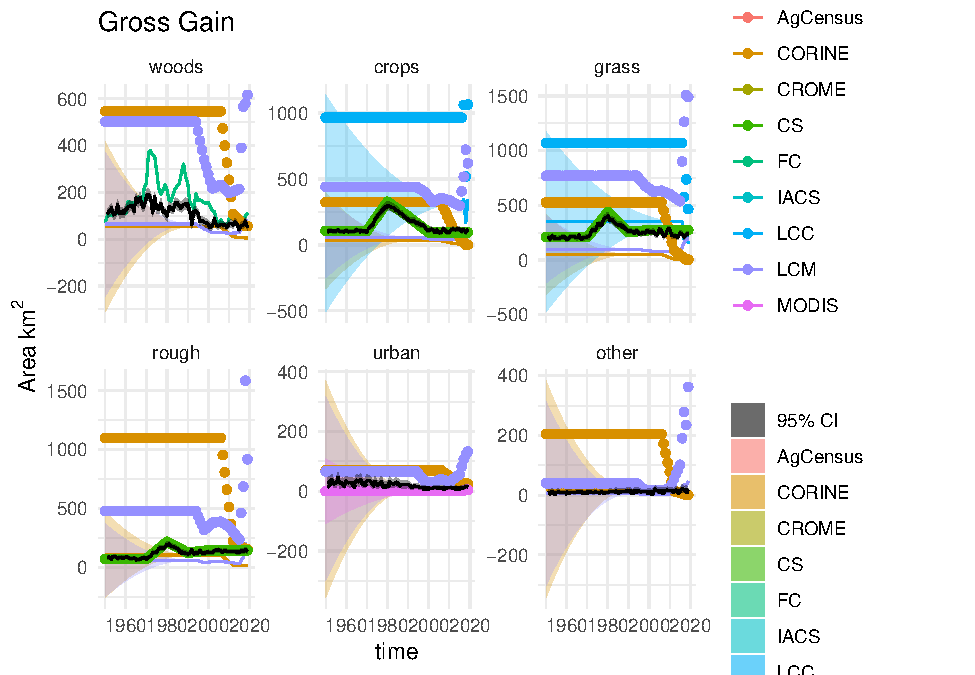
\includegraphics[width=1.3\linewidth]{Results_sc_files/figure-latex/plotG-1} \caption{ Observations and posterior distribution of the gross gain in area of each land use $\mathbf{G}$ from 1950 to 2020.  The grey shaded band shows the 2.5 and 97.5 percentiles of the posterior distribution. The maximum *a posteriori* estimate is shown as the solid black line within this. Observations from the different data sources are shown as coloured circles. The coloured solid lines show the corrected observations after accounting for systematic uncertainties, and interpolating. The coloured bands around these lines show the random uncertainty, rescaled as $\sigma /5$ to keep with the axis scale. Because the random uncertainties and the corrections to the observations are generally very large in comparison to the actual change, scaling the axes is difficult. Note that a consistent colour scheme for the data sources is shown, but not all contribute to every figure.}\label{fig:plotG}
\end{figure}

\begin{figure}
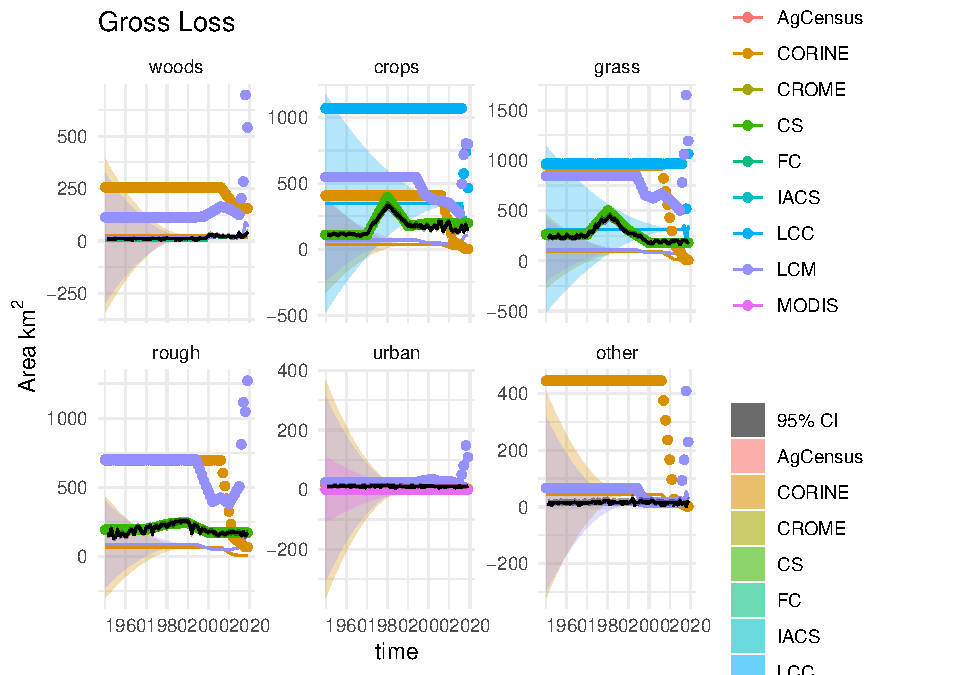
\includegraphics[width=1.3\linewidth]{Results_sc_files/figure-latex/plotL-1} \caption{ Observations and posterior distribution of the gross loss of area from each land use $\mathbf{L}$ from 1950 to 2020.  The grey shaded band shows the 2.5 and 97.5 percentiles of the posterior distribution. The maximum *a posteriori* estimate is shown as the solid black line within this. Observations from the different data sources are shown as coloured circles. The coloured solid lines show the corrected observations after accounting for systematic uncertainties, and interpolating. The coloured bands around these lines show the random uncertainty, rescaled as $\sigma /5$ to keep with the axis scale. Because the random uncertainties and the corrections to the observations are generally very large in comparison to the actual change, scaling the axes is difficult. Note that a consistent colour scheme for the data sources is shown, but not all contribute to every figure.}\label{fig:plotL}
\end{figure}

\begin{figure}
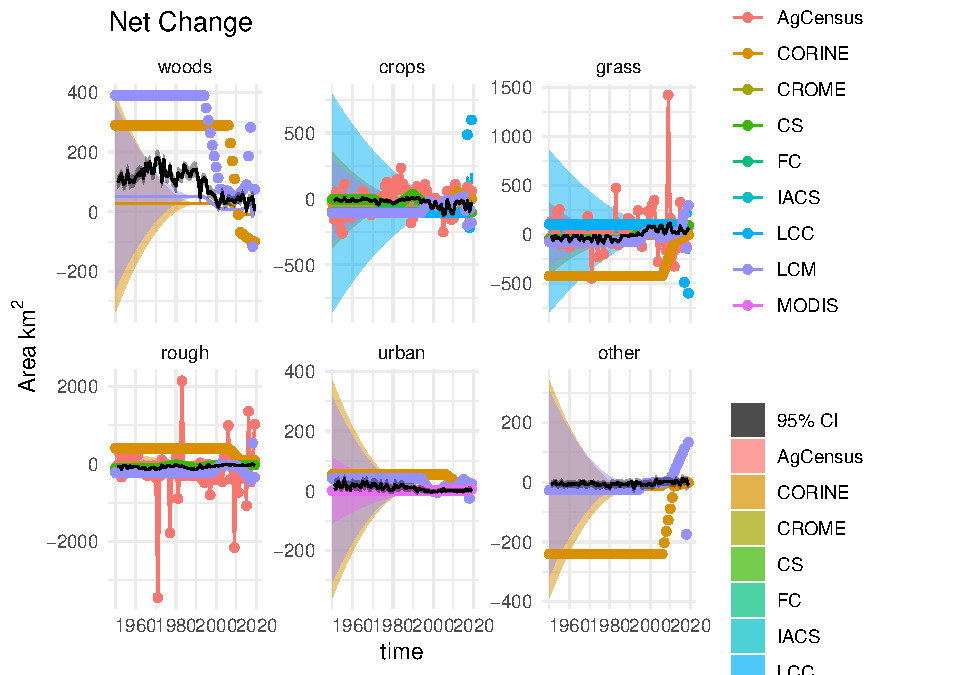
\includegraphics[width=1.3\linewidth]{Results_sc_files/figure-latex/plotD-1} \caption{ Time series of the net change in area occupied by each land use ($D$) from 1950 to 2020, showing the observations and posterior distribution of estimates. The grey shaded band shows the 2.5 and 97.5 percentiles of the posterior distribution. The maximum *a posteriori* estimate is shown as the solid black line within this. Observations from the different data sources are shown as coloured circles. The coloured solid lines show the corrected observations after accounting for systematic uncertainties, and interpolating. The coloured bands around these lines show the random uncertainty, rescaled as $\sigma /5$ to keep with the axis scale. Because the random uncertainties and the corrections to the observations are generally very large in comparison to the actual change, scaling the axes is difficult. Note that a consistent colour scheme for the data sources is shown, but not all contribute to every figure.}\label{fig:plotD}
\end{figure}

\begin{figure}
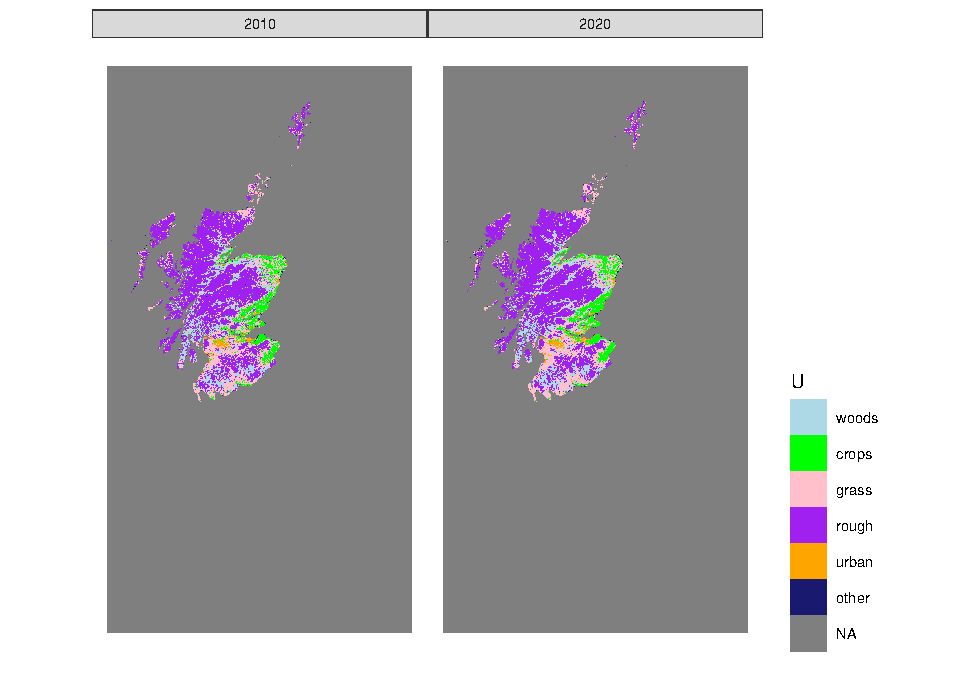
\includegraphics[width=1.3\linewidth]{Results_sc_files/figure-latex/plotUt-1} \caption{Estimated state of land-use in 2010 and 2020 in one realisation of $U$ from the maximum *a posteriori* estimate of $B$.}\label{fig:plotUt}
\end{figure}

\begin{figure}
\centering
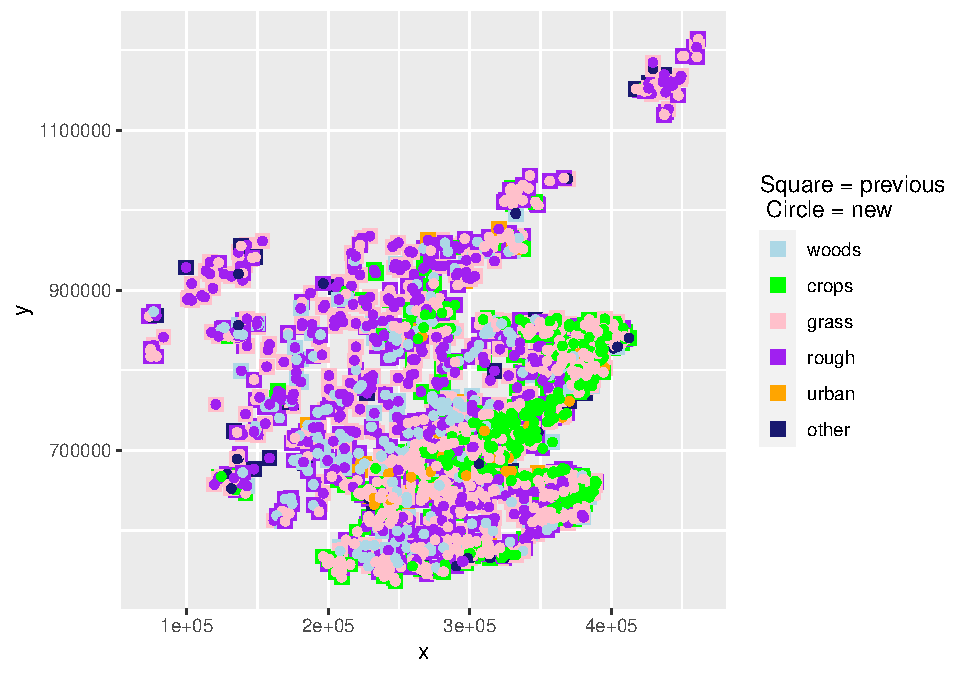
\includegraphics{Results_sc_files/figure-latex/plotUd-1.pdf}
\caption{\label{fig:plotUd}The spatial distribution of land-use change between 2010 and 2020 in one realisation of \(U\) from the maximum \emph{a posteriori} estimate of \(B\). At each location where land use has changed, the use in 2010 is shown as a coloured square, and the use in 2020 is shown as a coloured circle within this}
\end{figure}

\begin{figure}
\centering
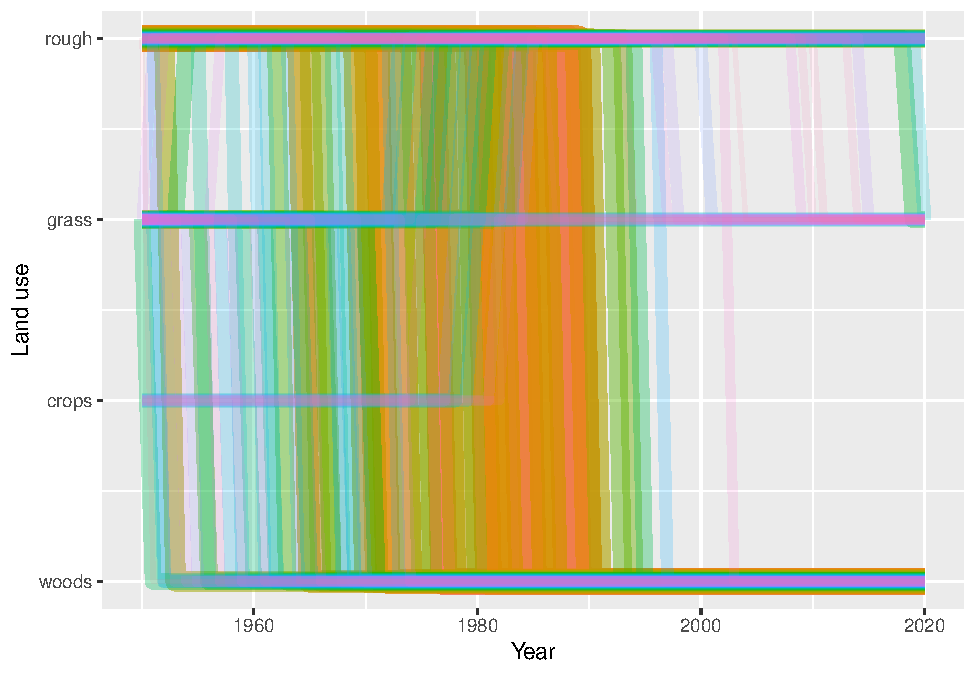
\includegraphics{Results_sc_files/figure-latex/plotv1-1.pdf}
\caption{\label{fig:plotv1}Trajectories of the 100 land-use vectors in the posterior \(U\) with the largest areas (excluding the six vectors which show no change). Each vector of land use is shown in a different colour, varied arbitrarily to differentiate different vectors. Line thickness and opacity are proportional to the total area occupied by each vector, so that the dominant vectors are the most visually obvious.}
\end{figure}

\begin{figure}
\centering
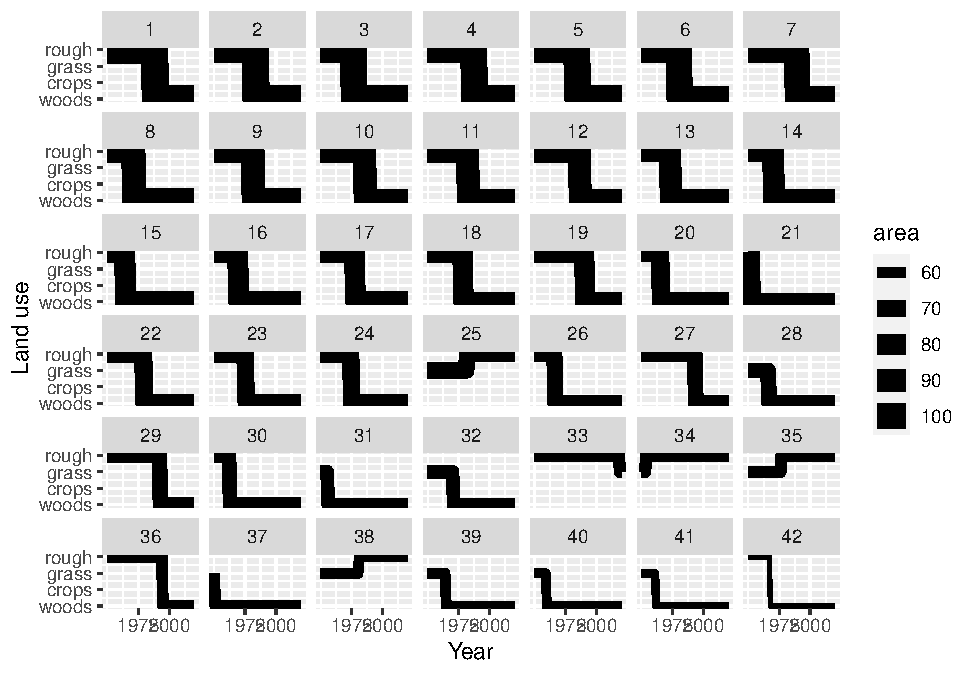
\includegraphics{Results_sc_files/figure-latex/plotv2-1.pdf}
\caption{\label{fig:plotv2}Trajectories of the 42 land-use vectors in the posterior \(U\) with the largest areas (excluding the six vectors which show no change). Line thickness is proportional to the total area occupied by each vector.}
\end{figure}

\begin{figure}
\centering
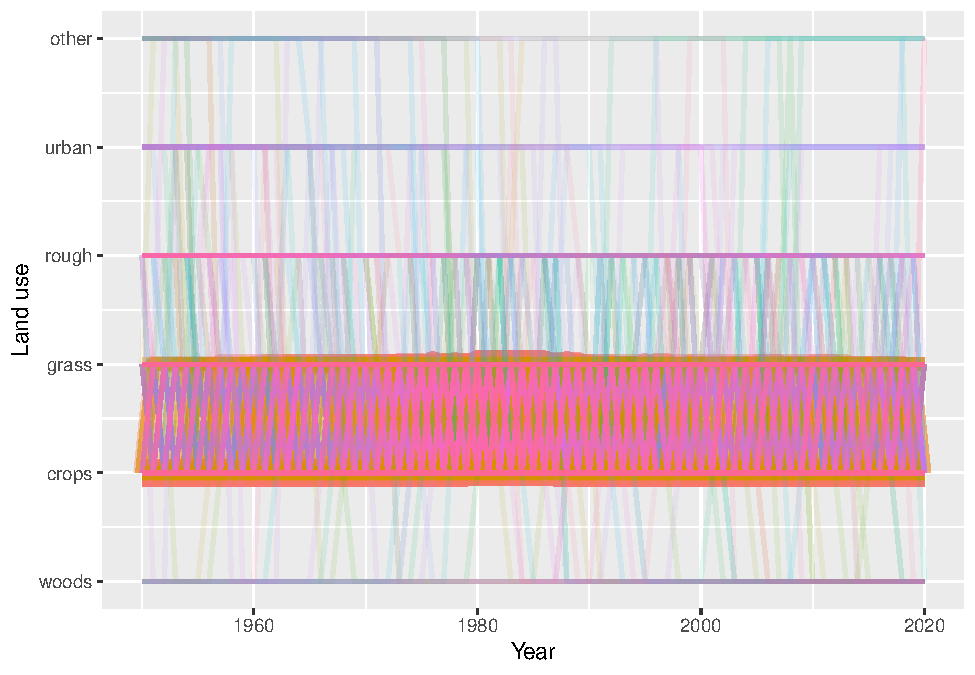
\includegraphics{Results_sc_files/figure-latex/plotcgr-1.pdf}
\caption{\label{fig:plotcgr}Trajectories of the land-use vectors in the posterior \(U\) which involve rotational change between crop and grassland (i.e.~those which include either (i) transitions from crop to grass and then subsequently from grass to crop, \emph{or} (ii) transitions from grass to crop and then subsequently from crop to grass). Each vector of land use is shown in a different colour, varied arbitrarily to differentiate different vectors. Line thickness and opacity are proportional to the total area occupied by each vector, so that the dominant vectors are the most visually obvious.}
\end{figure}

\hypertarget{results-wales}{%
\chapter{Results: Wales}\label{results-wales}}

The figures below show the results of the data assimilation procedure. All the data sets shown were used in the algorithm, but their relative random uncertainties (\(\sigma\)) determined how much influence they have on the estimates. The spatial data sets were corrected for systematic uncertainties, using the estimated net false positive rate (\(F_P\)). Having estimated the posterior distribution of the \(\beta\) matrix, we used this to simulate multiple maps of land use going back in time to 1950. The maps of the likelihood of transition to each land use established in WP-A were updated dynamically, using the life tables described in Section 5.

\begin{figure}
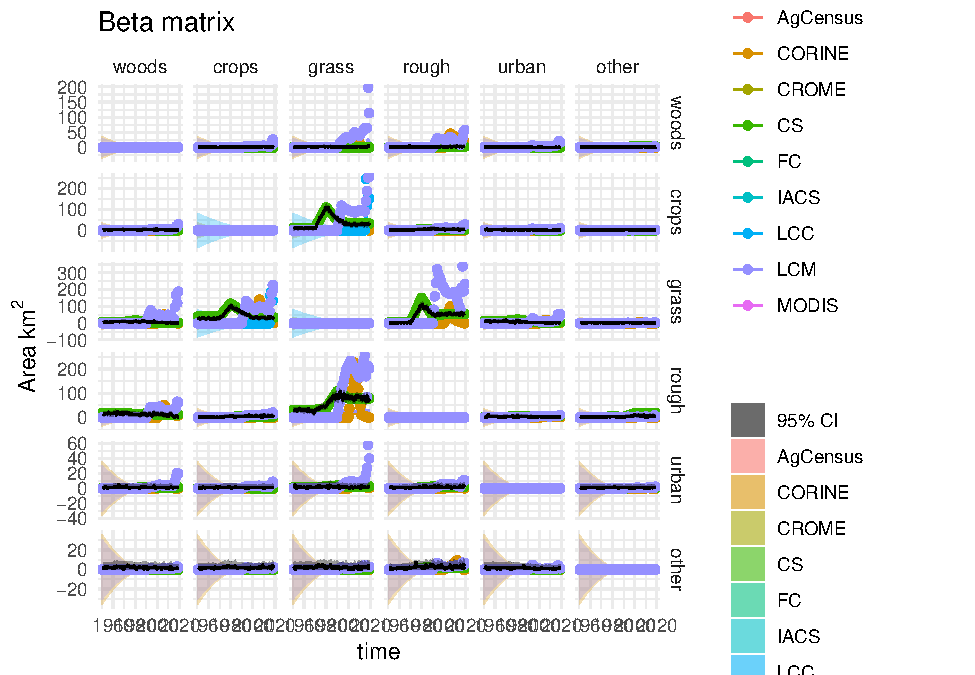
\includegraphics[width=1.3\linewidth]{Results_wa_files/figure-latex/plotB-1} \caption{ Observations and posterior distribution of the transition matrix $\mathbf{B}$, representing the gross area changing from the land use in each row to the land use in each column each year from 1950 to 2020. The grey shaded band shows the 2.5 and 97.5 percentiles of the posterior distribution. The maximum *a posteriori* estimate is shown as the solid black line within this. Observations from the different data sources are shown as coloured circles. The coloured solid lines show the corrected observations after accounting for systematic uncertainties, and interpolating. The coloured bands around these lines show the random uncertainty, rescaled as $\sigma /5$ to keep with the axis scale. Because the random uncertainties and the corrections to the observations are generally very large in comparison to the actual change, scaling the axes is difficult. Note that a consistent colour scheme for the data sources is shown, but not all contribute to every figure.}\label{fig:plotB}
\end{figure}

\begin{figure}
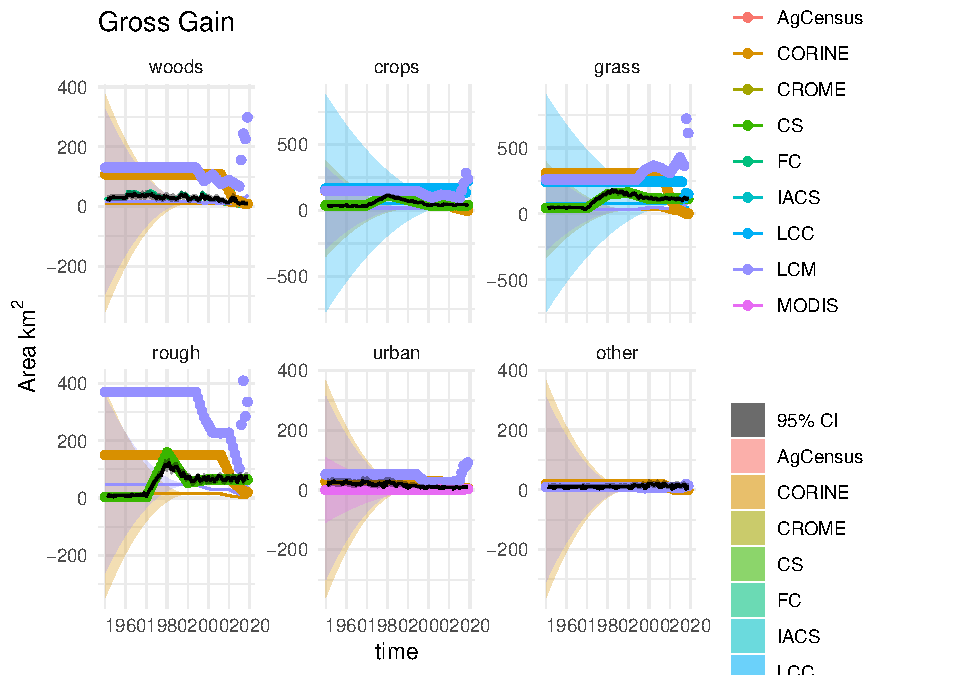
\includegraphics[width=1.3\linewidth]{Results_wa_files/figure-latex/plotG-1} \caption{ Observations and posterior distribution of the gross gain in area of each land use $\mathbf{G}$ from 1950 to 2020.  The grey shaded band shows the 2.5 and 97.5 percentiles of the posterior distribution. The maximum *a posteriori* estimate is shown as the solid black line within this. Observations from the different data sources are shown as coloured circles. The coloured solid lines show the corrected observations after accounting for systematic uncertainties, and interpolating. The coloured bands around these lines show the random uncertainty, rescaled as $\sigma /5$ to keep with the axis scale. Because the random uncertainties and the corrections to the observations are generally very large in comparison to the actual change, scaling the axes is difficult. Note that a consistent colour scheme for the data sources is shown, but not all contribute to every figure.}\label{fig:plotG}
\end{figure}

\begin{figure}
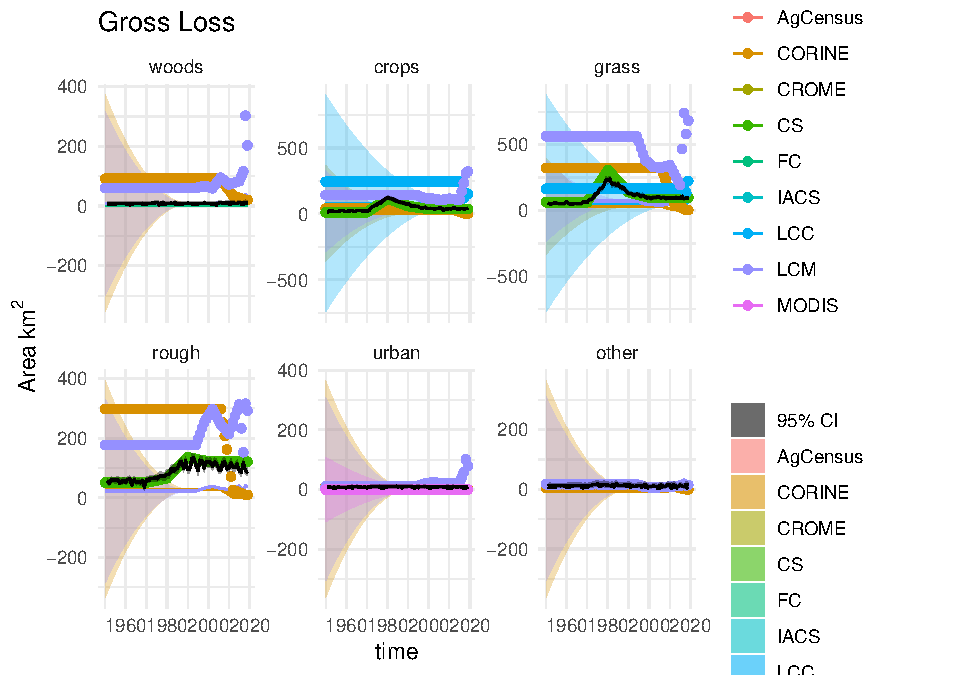
\includegraphics[width=1.3\linewidth]{Results_wa_files/figure-latex/plotL-1} \caption{ Observations and posterior distribution of the gross loss of area from each land use $\mathbf{L}$ from 1950 to 2020.  The grey shaded band shows the 2.5 and 97.5 percentiles of the posterior distribution. The maximum *a posteriori* estimate is shown as the solid black line within this. Observations from the different data sources are shown as coloured circles. The coloured solid lines show the corrected observations after accounting for systematic uncertainties, and interpolating. The coloured bands around these lines show the random uncertainty, rescaled as $\sigma /5$ to keep with the axis scale. Because the random uncertainties and the corrections to the observations are generally very large in comparison to the actual change, scaling the axes is difficult. Note that a consistent colour scheme for the data sources is shown, but not all contribute to every figure.}\label{fig:plotL}
\end{figure}

\begin{figure}
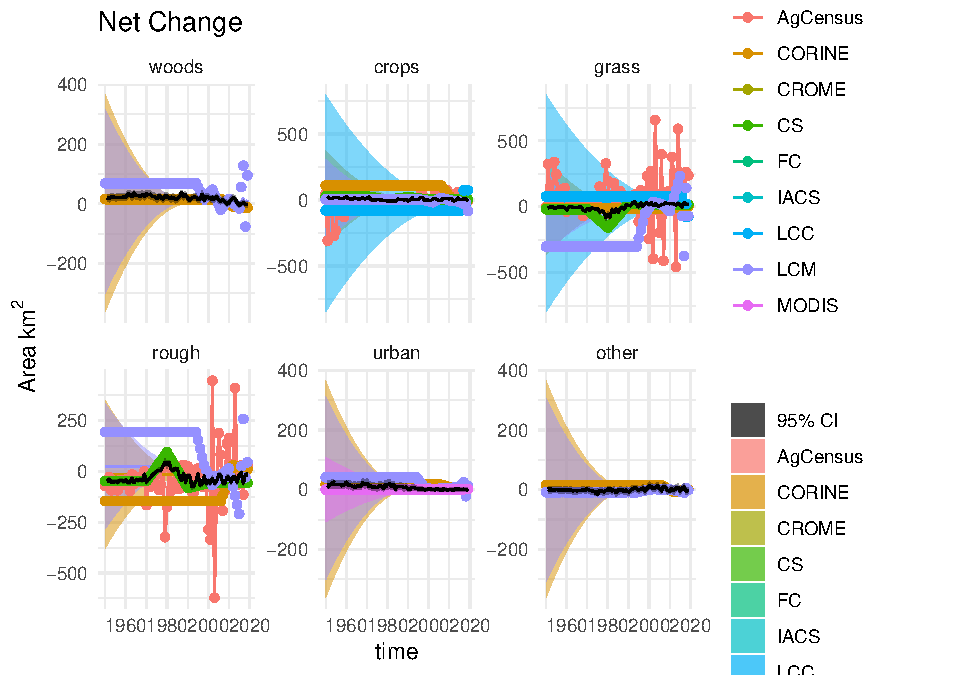
\includegraphics[width=1.3\linewidth]{Results_wa_files/figure-latex/plotD-1} \caption{ Time series of the net change in area occupied by each land use ($D$) from 1950 to 2020, showing the observations and posterior distribution of estimates. The grey shaded band shows the 2.5 and 97.5 percentiles of the posterior distribution. The maximum *a posteriori* estimate is shown as the solid black line within this. Observations from the different data sources are shown as coloured circles. The coloured solid lines show the corrected observations after accounting for systematic uncertainties, and interpolating. The coloured bands around these lines show the random uncertainty, rescaled as $\sigma /5$ to keep with the axis scale. Because the random uncertainties and the corrections to the observations are generally very large in comparison to the actual change, scaling the axes is difficult. Note that a consistent colour scheme for the data sources is shown, but not all contribute to every figure.}\label{fig:plotD}
\end{figure}

\begin{figure}
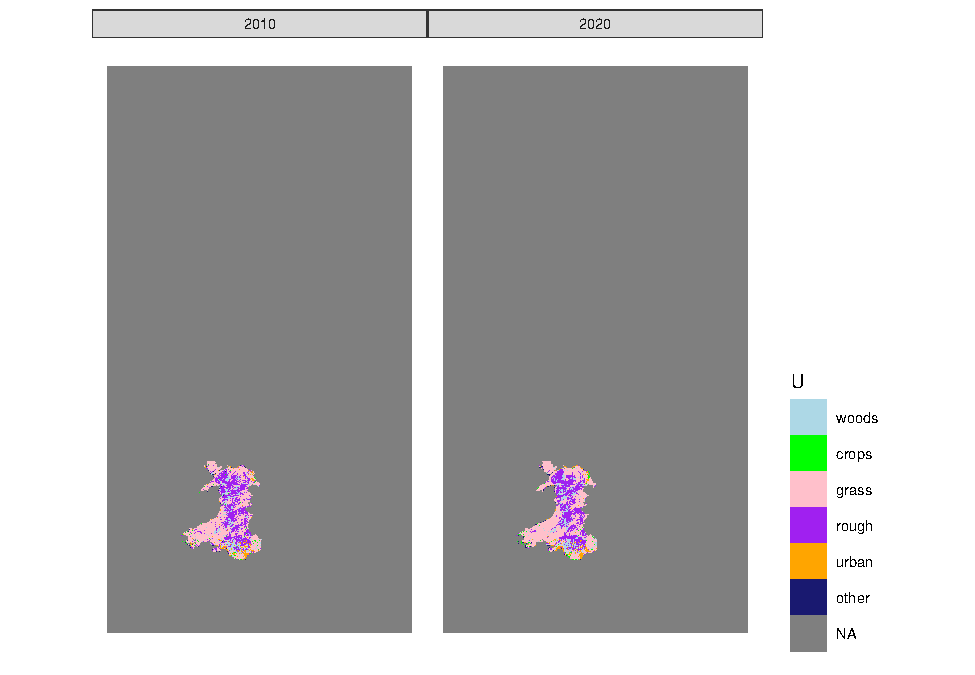
\includegraphics[width=1.3\linewidth]{Results_wa_files/figure-latex/plotUt-1} \caption{Estimated state of land-use in 2010 and 2020 in one realisation of $U$ from the maximum *a posteriori* estimate of $B$.}\label{fig:plotUt}
\end{figure}

\begin{figure}
\centering
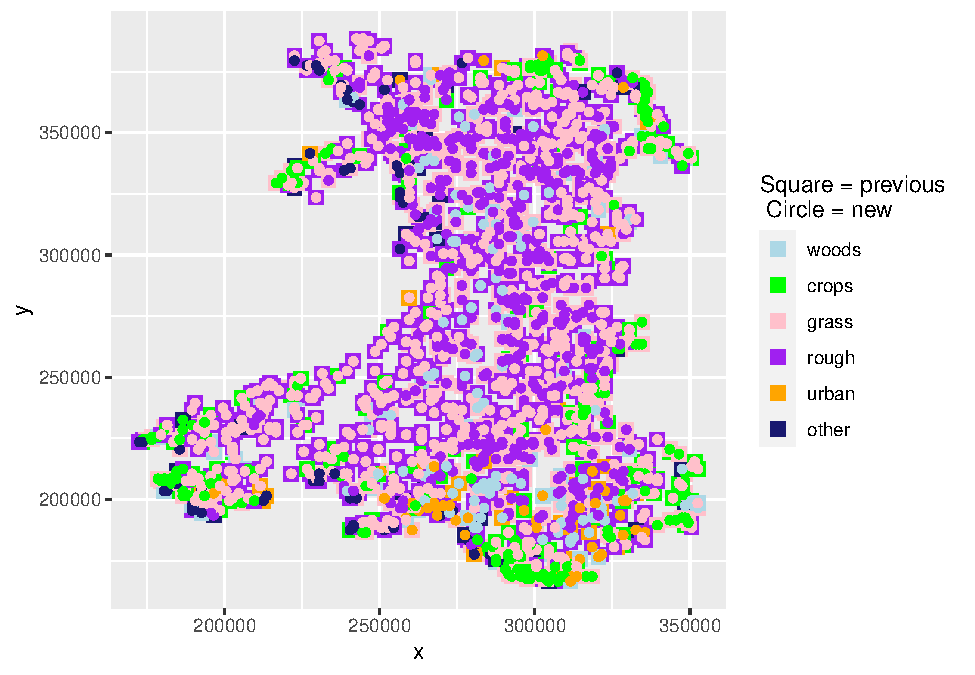
\includegraphics{Results_wa_files/figure-latex/plotUd-1.pdf}
\caption{\label{fig:plotUd}The spatial distribution of land-use change between 2010 and 2020 in one realisation of \(U\) from the maximum \emph{a posteriori} estimate of \(B\). At each location where land use has changed, the use in 2010 is shown as a coloured square, and the use in 2020 is shown as a coloured circle within this}
\end{figure}

\begin{figure}
\centering
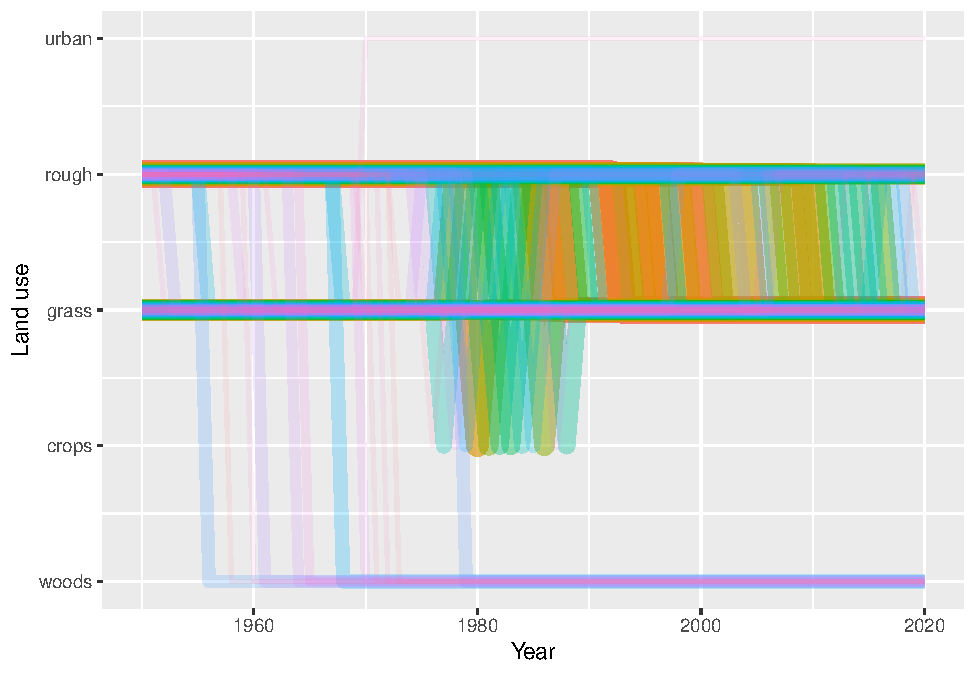
\includegraphics{Results_wa_files/figure-latex/plotv1-1.pdf}
\caption{\label{fig:plotv1}Trajectories of the 100 land-use vectors in the posterior \(U\) with the largest areas (excluding the six vectors which show no change). Each vector of land use is shown in a different colour, varied arbitrarily to differentiate different vectors. Line thickness and opacity are proportional to the total area occupied by each vector, so that the dominant vectors are the most visually obvious.}
\end{figure}

\begin{figure}
\centering
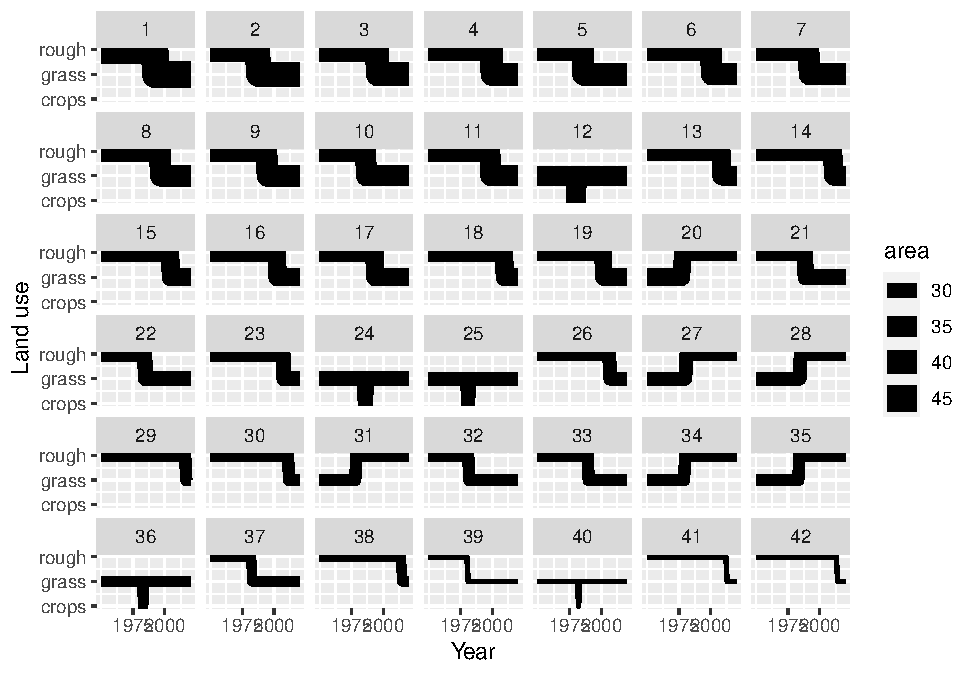
\includegraphics{Results_wa_files/figure-latex/plotv2-1.pdf}
\caption{\label{fig:plotv2}Trajectories of the 42 land-use vectors in the posterior \(U\) with the largest areas (excluding the six vectors which show no change). Line thickness is proportional to the total area occupied by each vector.}
\end{figure}

\begin{figure}
\centering
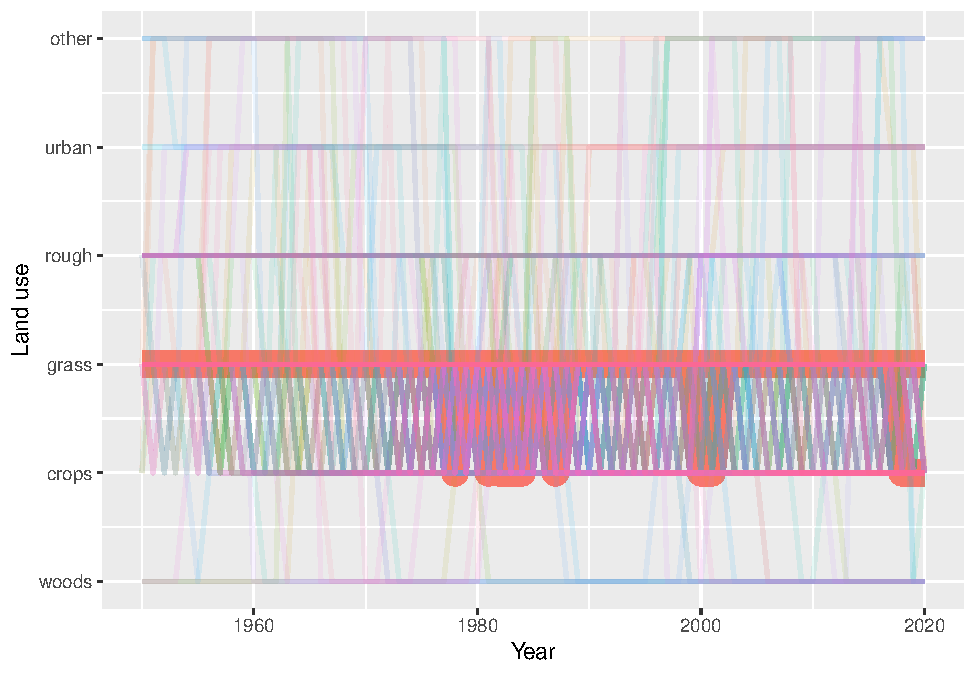
\includegraphics{Results_wa_files/figure-latex/plotcgr-1.pdf}
\caption{\label{fig:plotcgr}Trajectories of the land-use vectors in the posterior \(U\) which involve rotational change between crop and grassland (i.e.~those which include either (i) transitions from crop to grass and then subsequently from grass to crop, \emph{or} (ii) transitions from grass to crop and then subsequently from crop to grass). Each vector of land use is shown in a different colour, varied arbitrarily to differentiate different vectors. Line thickness and opacity are proportional to the total area occupied by each vector, so that the dominant vectors are the most visually obvious.}
\end{figure}

\hypertarget{results-northern-ireland}{%
\chapter{Results: Northern Ireland}\label{results-northern-ireland}}

The figures below show the results of the data assimilation procedure. All the data sets shown were used in the algorithm, but their relative random uncertainties (\(\sigma\)) determined how much influence they have on the estimates. The spatial data sets were corrected for systematic uncertainties, using the estimated net false positive rate (\(F_P\)). Having estimated the posterior distribution of the \(\beta\) matrix, we used this to simulate multiple maps of land use going back in time to 1950. The maps of the likelihood of transition to each land use established in WP-A were updated dynamically, using the life tables described in Section 5.

\begin{figure}
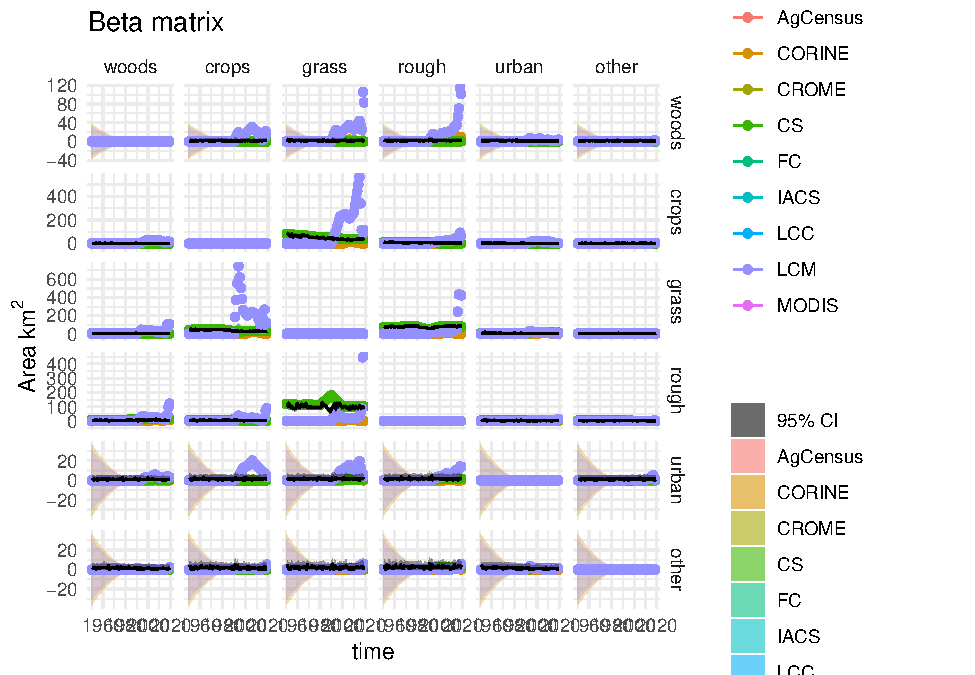
\includegraphics[width=1.3\linewidth]{Results_ni_files/figure-latex/plotB-1} \caption{ Observations and posterior distribution of the transition matrix $\mathbf{B}$, representing the gross area changing from the land use in each row to the land use in each column each year from 1950 to 2020. The grey shaded band shows the 2.5 and 97.5 percentiles of the posterior distribution. The maximum *a posteriori* estimate is shown as the solid black line within this. Observations from the different data sources are shown as coloured circles. The coloured solid lines show the corrected observations after accounting for systematic uncertainties, and interpolating. The coloured bands around these lines show the random uncertainty, rescaled as $\sigma /5$ to keep with the axis scale. Because the random uncertainties and the corrections to the observations are generally very large in comparison to the actual change, scaling the axes is difficult. Note that a consistent colour scheme for the data sources is shown, but not all contribute to every figure.}\label{fig:plotB}
\end{figure}

\begin{figure}
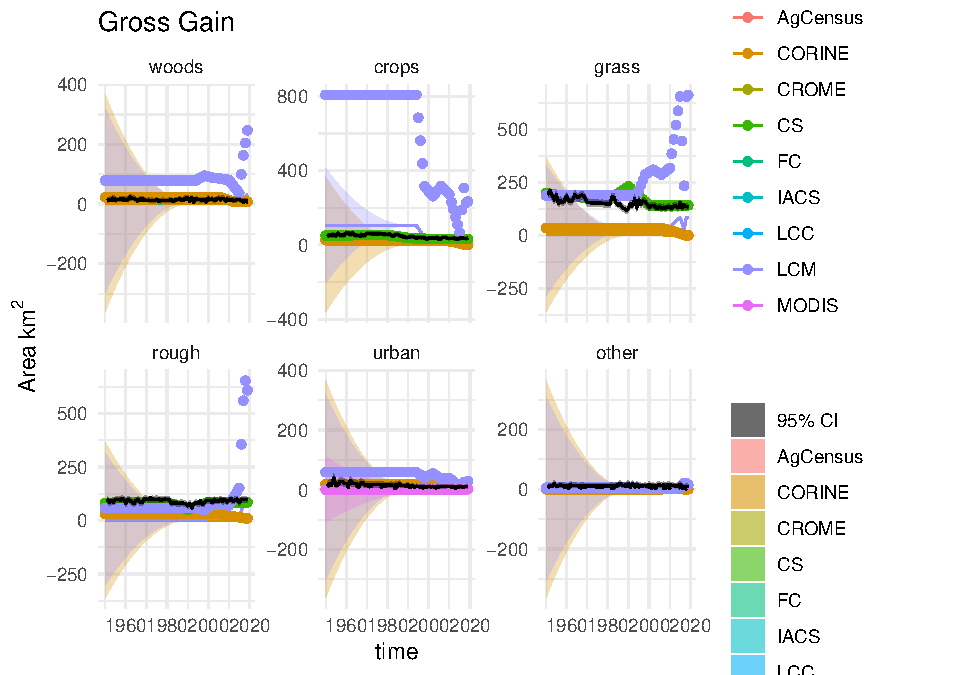
\includegraphics[width=1.3\linewidth]{Results_ni_files/figure-latex/plotG-1} \caption{ Observations and posterior distribution of the gross gain in area of each land use $\mathbf{G}$ from 1950 to 2020.  The grey shaded band shows the 2.5 and 97.5 percentiles of the posterior distribution. The maximum *a posteriori* estimate is shown as the solid black line within this. Observations from the different data sources are shown as coloured circles. The coloured solid lines show the corrected observations after accounting for systematic uncertainties, and interpolating. The coloured bands around these lines show the random uncertainty, rescaled as $\sigma /5$ to keep with the axis scale. Because the random uncertainties and the corrections to the observations are generally very large in comparison to the actual change, scaling the axes is difficult. Note that a consistent colour scheme for the data sources is shown, but not all contribute to every figure.}\label{fig:plotG}
\end{figure}

\begin{figure}
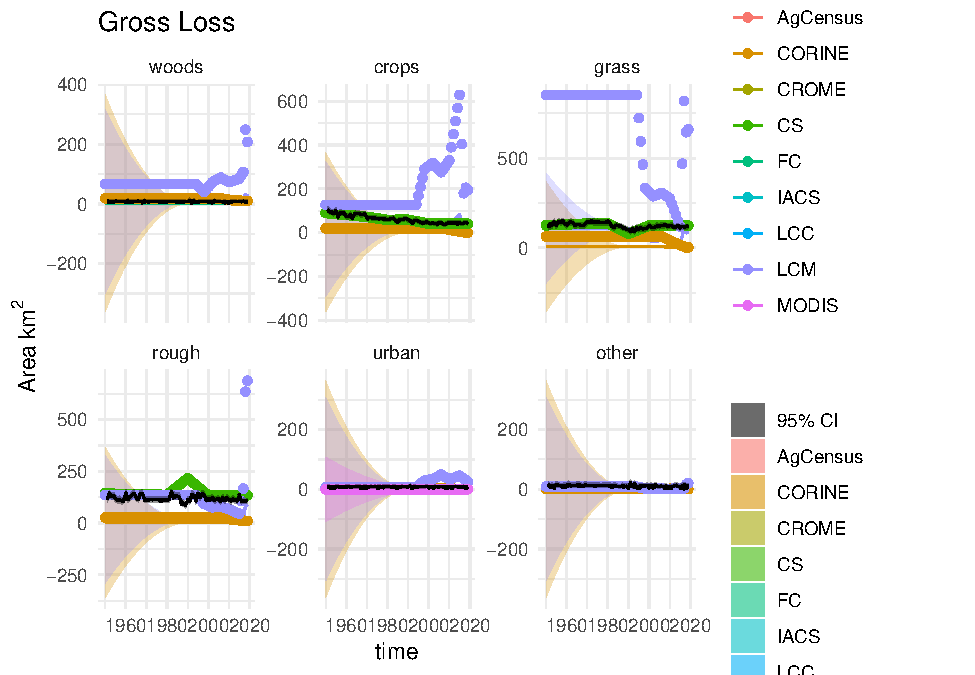
\includegraphics[width=1.3\linewidth]{Results_ni_files/figure-latex/plotL-1} \caption{ Observations and posterior distribution of the gross loss of area from each land use $\mathbf{L}$ from 1950 to 2020.  The grey shaded band shows the 2.5 and 97.5 percentiles of the posterior distribution. The maximum *a posteriori* estimate is shown as the solid black line within this. Observations from the different data sources are shown as coloured circles. The coloured solid lines show the corrected observations after accounting for systematic uncertainties, and interpolating. The coloured bands around these lines show the random uncertainty, rescaled as $\sigma /5$ to keep with the axis scale. Because the random uncertainties and the corrections to the observations are generally very large in comparison to the actual change, scaling the axes is difficult. Note that a consistent colour scheme for the data sources is shown, but not all contribute to every figure.}\label{fig:plotL}
\end{figure}

\begin{figure}
\centering
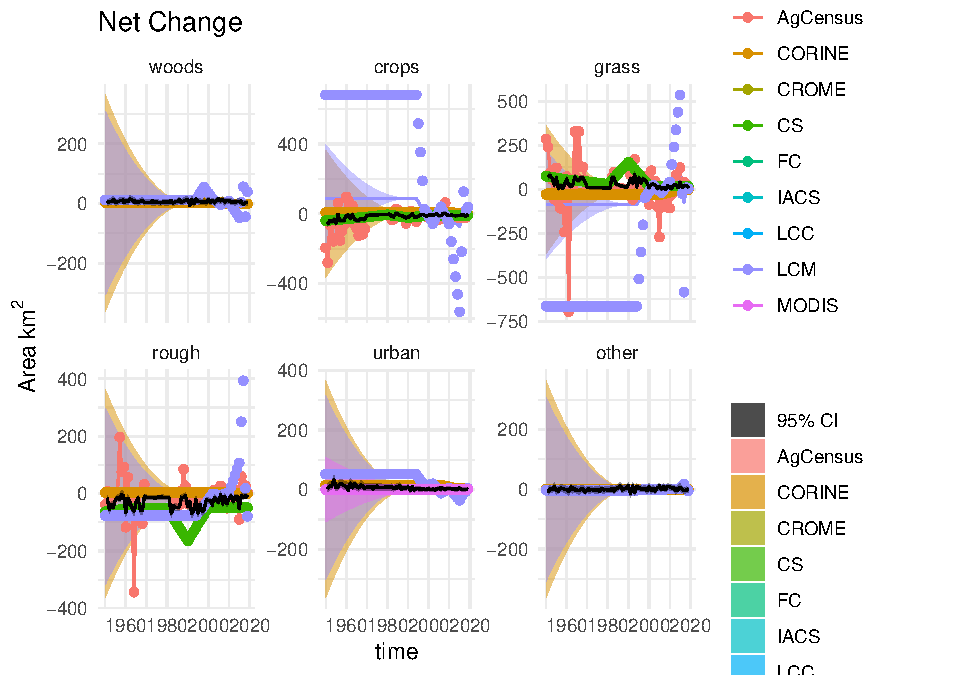
\includegraphics{Results_ni_files/figure-latex/plotD-1.pdf}
\caption{\label{fig:plotD} Time series of the net change in area occupied by each land use (\(D\)) from 1950 to 2020, showing the observations and posterior distribution of estimates. The grey shaded band shows the 2.5 and 97.5 percentiles of the posterior distribution. The maximum \emph{a posteriori} estimate is shown as the solid black line within this. Observations from the different data sources are shown as coloured circles. The coloured solid lines show the corrected observations after accounting for systematic uncertainties, and interpolating. The coloured bands around these lines show the random uncertainty, rescaled as \(\sigma /5\) to keep with the axis scale. Because the random uncertainties and the corrections to the observations are generally very large in comparison to the actual change, scaling the axes is difficult. Note that a consistent colour scheme for the data sources is shown, but not all contribute to every figure.}
\end{figure}

\begin{figure}
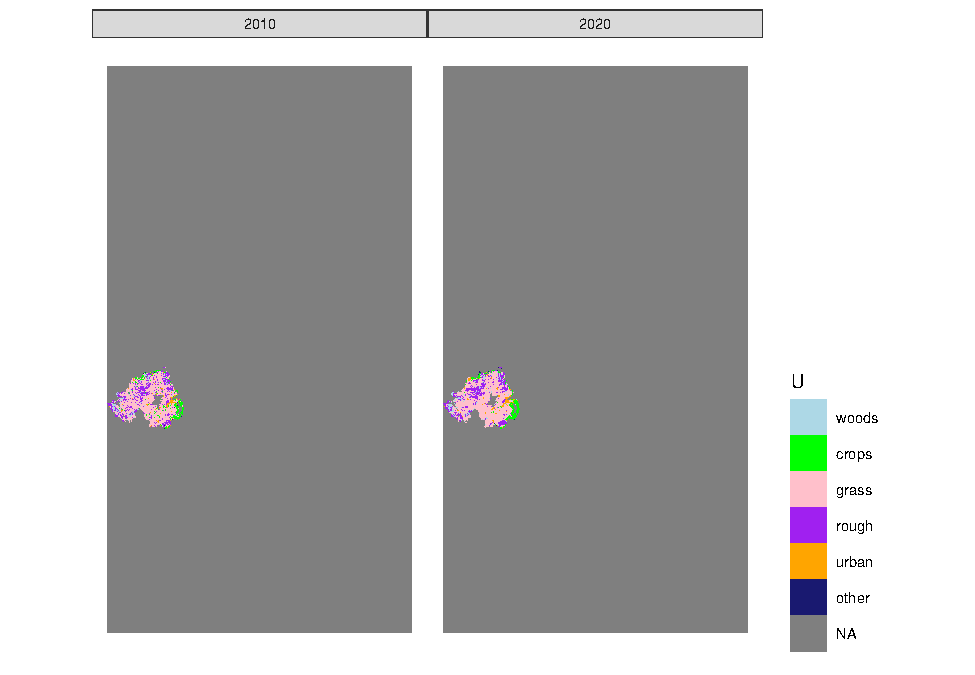
\includegraphics[width=1.3\linewidth]{Results_ni_files/figure-latex/plotUt-1} \caption{Estimated state of land-use in 2010 and 2020 in one realisation of $U$ from the maximum *a posteriori* estimate of $B$.}\label{fig:plotUt}
\end{figure}

\begin{figure}
\centering
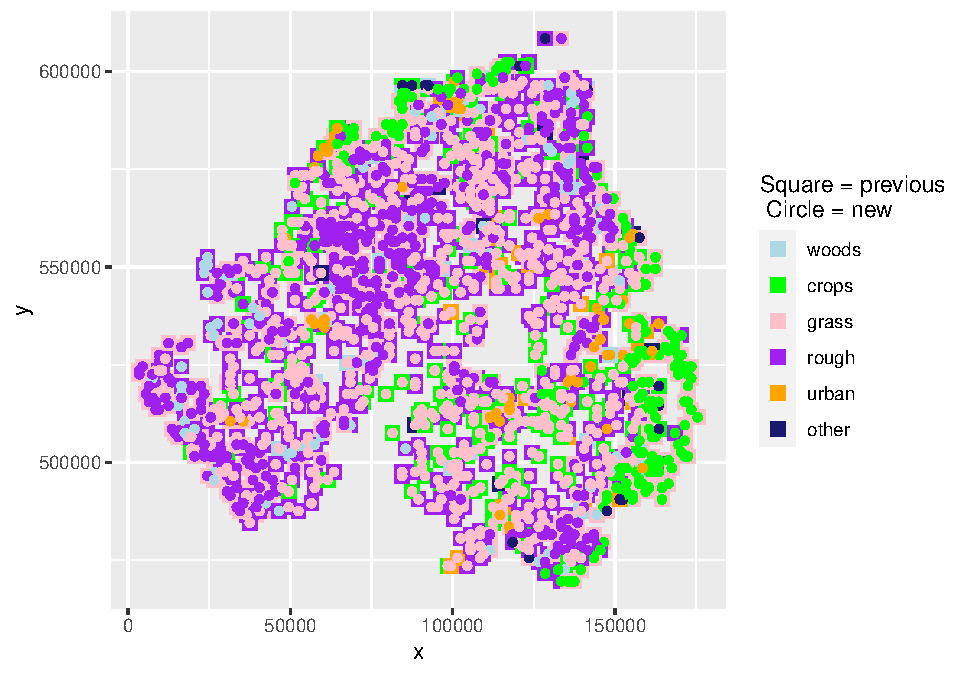
\includegraphics{Results_ni_files/figure-latex/plotUd-1.pdf}
\caption{\label{fig:plotUd}The spatial distribution of land-use change between 2010 and 2020 in one realisation of \(U\) from the maximum \emph{a posteriori} estimate of \(B\). At each location where land use has changed, the use in 2010 is shown as a coloured square, and the use in 2020 is shown as a coloured circle within this}
\end{figure}

\begin{figure}
\centering
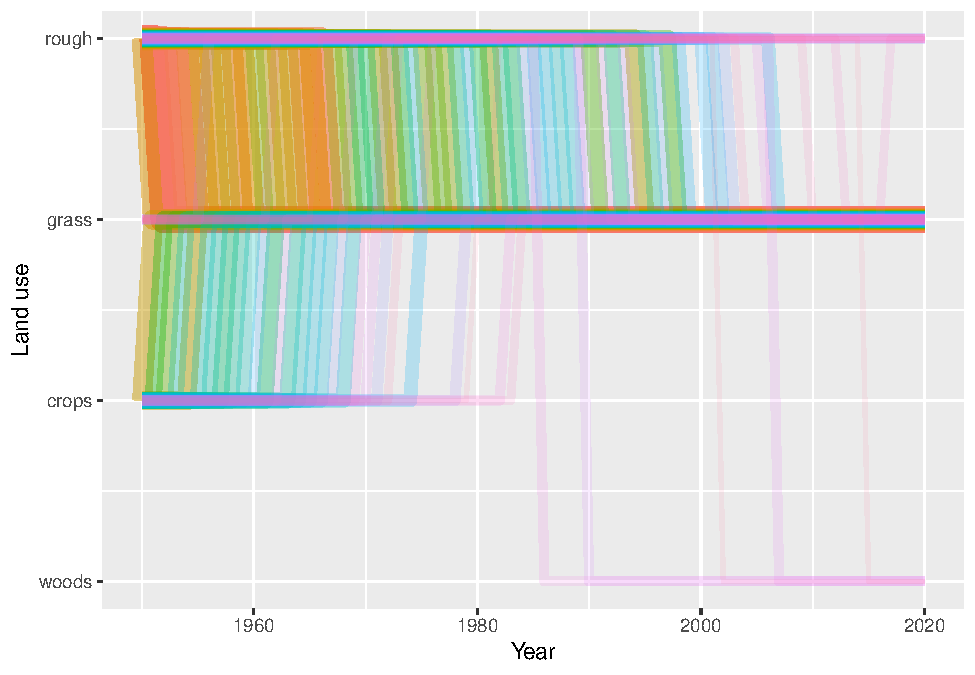
\includegraphics{Results_ni_files/figure-latex/plotv1-1.pdf}
\caption{\label{fig:plotv1}Trajectories of the 100 land-use vectors in the posterior \(U\) with the largest areas (excluding the six vectors which show no change). Each vector of land use is shown in a different colour, varied arbitrarily to differentiate different vectors. Line thickness and opacity are proportional to the total area occupied by each vector, so that the dominant vectors are the most visually obvious.}
\end{figure}

\begin{figure}
\centering
\includegraphics{Results_ni_files/figure-latex/plotv2-1.pdf}
\caption{\label{fig:plotv2}Trajectories of the 42 land-use vectors in the posterior \(U\) with the largest areas (excluding the six vectors which show no change). Line thickness is proportional to the total area occupied by each vector.}
\end{figure}

\begin{figure}
\centering
\includegraphics{Results_ni_files/figure-latex/plotcgr-1.pdf}
\caption{\label{fig:plotcgr}Trajectories of the land-use vectors in the posterior \(U\) which involve rotational change between crop and grassland (i.e.~those which include either (i) transitions from crop to grass and then subsequently from grass to crop, \emph{or} (ii) transitions from grass to crop and then subsequently from crop to grass). Each vector of land use is shown in a different colour, varied arbitrarily to differentiate different vectors. Line thickness and opacity are proportional to the total area occupied by each vector, so that the dominant vectors are the most visually obvious.}
\end{figure}

\hypertarget{refs}{}
\leavevmode\hypertarget{ref-Levy2018}{}%
Levy, P., M. van Oijen, G. Buys, and S. Tomlinson. 2018. ``Estimation of Gross Land-Use Change and Its Uncertainty Using a Bayesian Data Assimilation Approach.'' \emph{Biogeosciences} 15 (5): 1497--1513. \url{https://doi.org/10.5194/bg-15-1497-2018}.

\end{document}
